% ============================================================
% slides3.tex: talk for experimentalists (2026-11-03).
% Built from slides2.tex: the intro frames up to the microscopic model are kept; Dean's
% equation is stated, not derived; the results follow manuscript/manuscript.tex
% (parameters of its App. A). Every number on a result frame is taken from manuscript.tex.
%
% Colour code: blue = interactions, red = self-propulsion & reversals, green = rotational
% noise; on the Dean frames green = noise, orange = Ito term / entropy (as in slides2).
% Every frame carries a \note{} with what to say; [m:ss] = time for the frame.
%
% Build (from slides/):
%   latexmk -f -pdf -outdir=.tmp slides3.tex        && cp .tmp/slides3.pdf .
%   latexmk -f -pdf -outdir=.tmp slides3-notes.tex  && cp .tmp/slides3-notes.pdf .
% (-f because bibtex stops on the duplicate key dean1996 in literature.bib.)
% ============================================================
\documentclass[12pt,aspectratio=169]{beamer}

\usepackage{amsmath,amssymb}
\usepackage{graphicx}
\usepackage[english]{babel}
\usepackage{ragged2e}
\usepackage{cancel}
\usepackage{tikz}
\usetikzlibrary{arrows.meta,decorations.pathmorphing,positioning,calc}
\usepackage{textcomp}
\usepackage{silence}
\usepackage{catchfile}
\usepackage{ifthen}
\usepackage{upgreek}
\usepackage{booktabs}
\usepackage{array}
\usepackage{animate}
\usepackage{pgfpages}
\usepackage{appendixnumberbeamer}

\usepackage[backend=bibtex]{biblatex}
\addbibresource{literature.bib}

\usepackage{mathtools}
\mathtoolsset{showonlyrefs}



\renewcommand{\CancelColor}{\color{red}} %change cancel color to red

\makeatletter
\let\my@cancelto\cancelto %copy over the original cancelto command
\newcommand<>{\cancelto}[2]{\alt#3{\my@cancelto{#1}{#2}}{\mathrlap{#2}\phantom{\my@cancelto{#1}{#2}}}}
% redefine the cancelto command, using \phantom to assure that the
% result doesn't wiggle up and down with and without the arrow
\makeatother



\newenvironment{wide}[1]{\begin{columns}\column{\dimexpr\paperwidth-#1}}{\end{columns}}

\newenvironment{wide2}[2][1ex]{\begin{columns}\column{\dimexpr\paperwidth-#2}
\begin{minipage}[t][\textheight-#1]{\textwidth}
}{\end{minipage}\end{columns}}


% \definecolor{beamer@blendedblue}{rgb}{0.07,0.20,0.47}
% \setbeamercolor{structure}{fg=beamer@blendedblue}

\definecolor{bblue}{rgb}{0.2,0.2,0.7} % beamer blue
\definecolor{darkred}{rgb}{0.8,0,0}
\definecolor{litered}{rgb}{0.2,1,1}
\definecolor{Darkred}{rgb}{0.7,0,0}
\definecolor{liteyellow}{rgb}{1,1,0.7}
\definecolor{litegreen}{rgb}{0.8,1,0.8}
\definecolor{darkgreen}{rgb}{0,0.5,0}
\definecolor{litelitegray}{rgb}{0.8,0.8,0.8}
\definecolor{litegray}{rgb}{0.6,0.6,0.6}
\definecolor{purple}{rgb}{0.58,0,0.58}
\definecolor{darkmag}{rgb}{0.5,0.0,0.5}
\definecolor{darkorange}{rgb}{0.68,0.28,0.04}
\definecolor{darkbrown}{rgb}{0.55,0.35,0.15}





\newcommand<>{\altfixed}[2]{\alt#3{#1}{\mathrlap{#2}\phantom{#1}}}
\newcommand<>{\altfixedother}[2]{\alt#3{\mathrlap{#1}\phantom{#2}}{#2}}



\renewcommand<>{\mathcolorboxalt}[2]{
	\altfixed#3{{ \setlength{\fboxsep}{0pt} \colorbox{#1}{$\displaystyle #2$}}}{#2}
}




\renewcommand<>\hlbox[2]{%
  \alt#3{\colorbox{#1}{#2}}%
  {\makebox[\dimexpr\width+2\fboxsep]{#2}\vphantom{\colorbox{#1}{#2}}}%
}
\newcommand<>{\mathhlbox}[2]{%
	\alt#3{\colorbox{#1}{$\displaystyle #2$}}%
	{\makebox[\dimexpr\width+2\fboxsep]{$\displaystyle #2$}\vphantom{\colorbox{#1}{$\displaystyle #2$}}}%
}
\newcommand<>{\mathhlboxRGB}[2]{%
	\alt#3{\colorbox[RGB]{#1}{$\displaystyle #2$}}%
	{\makebox[\dimexpr\width+2\fboxsep]{$\displaystyle #2$}\vphantom{\colorbox[RGB]{#1}{$\displaystyle #2$}}}%
}
\newcommand<>{\hlboxRGB}[2]{%
	\alt#3{\colorbox[RGB]{#1}{#2}}%
	{\makebox[\dimexpr\width+2\fboxsep]{#2}\vphantom{\colorbox[RGB]{#1}{#2}}}%
}

\newcommand<>{\mathcolorbox}[2]{
	\alt#3{\colorbox{#1}{$\displaystyle #2$}}{\colorbox{white}{$\displaystyle #2$}}%
}
\newcommand<>{\mathcolorboxRGB}[2]{
	\alt#3{\colorbox[RGB]{#1}{$\displaystyle #2$}}{\colorbox{white}{$\displaystyle #2$}}%
}

\newcommand<>{\mathaltcolorbox}[3]{% color, expr1, expr2 
	\altfixed#4{\colorbox{#1}{$\displaystyle #2$}}{\colorbox{white}{$\displaystyle #3$}}%
}

% define backslash symbol $/$
\newcommand{\bsh}[0]{\textbackslash}




% hide navigation symbols
\setbeamertemplate{navigation symbols}{}
\addtobeamertemplate{navigation symbols}{}{%
	\usebeamerfont{footline}%
	\usebeamercolor[fg]{footline}%
	\hspace{1em}%
	\insertframenumber/\inserttotalframenumber
}

% make boxes rounded
\setbeamertemplate{blocks}[rounded][shadow=false]



% footnote without number
\addtobeamertemplate{footnote}{\hskip -2em}{}
\newcommand{\footnotetextrelaxed}[1]{{\let\thefootnote\relax\footnotetext{#1}}}


\usepackage{catchfile}


% \usepackage{catchfile}
% make animate work in Texpad compiler
\CatchFileDef{\CompilationMode}{mode.txt}{}
\ifthenelse{\equal{\CompilationMode}{make }}{}{
    \renewcommand{\animategraphics}[5][]{\ErrorsOff[xkeyval]\ErrorsOff[keyval]\includegraphics[#1]{#3#4}}
    }


\let\x\relax
\let\eszett\ss   % definitions.tex redefines \ss
% ============================================================
% definitions.tex — macros for manuscript.tex
%
% Carried over from the top-level derivation log (../definitions.tex),
% trimmed of nothing, plus a small block of new macros at the end for
% symbols introduced in the Extrusion/Nucleation section (dean.tex
% "Extrusion rate": Virtual work, The nucleation threshold, Layering
% probability) that did not exist when the derivation-log definitions
% file was written. Keep the two files in sync by hand — there is no
% automated check.
% ============================================================

\newcommand{\la}{\left\langle}
\newcommand{\ra}{\right\rangle}
\newcommand{\bs}{\boldsymbol}
\newcommand{\E}{\mathbf{E}}
\newcommand{\Var}{\text{Var}}
\renewcommand{\d}{\mathrm{d}}
\renewcommand{\u}{\bs{u}}
\newcommand{\q}{\bs{q}}
\newcommand{\Q}{\mathbf{Q}}
\newcommand{\R}{\mathbb{R}}
\newcommand{\n}{\bs{n}}
\newcommand{\e}{\bs{e}}
\newcommand{\T}[0]{\mathrm{T}}
\newcommand{\pd}[2]{\frac{\partial #1}{\partial #2}}
\newcommand{\tpd}[2]{\tfrac{\partial #1}{\partial #2}}


\newcommand{\ab}{{\alpha\beta}}
\newcommand{\mn}{{\mu\nu}}
\newcommand{\abmn}{{\alpha\beta\mu\nu}}

\newcommand{\eye}{\bs{\mathrm{I}}}
\renewcommand{\v}{\mathbf{v}}
\newcommand{\x}{\mathbf{x}}
\newcommand{\f}{\mathbf{f}}
\newcommand{\s}{\mathbf{s}}
\newcommand{\g}{\mathbf{g}}
\newcommand{\G}{\mathbf{G}}
\renewcommand{\H}{\mathbf{H}}
\newcommand{\Ha}{\mathbf{H}_\text{a}}
\newcommand{\F}{\mathbf{F}}
\newcommand{\I}{\mathbf{I}}
\newcommand{\J}{\mathbf{J}}
\newcommand{\bnabla}{\boldsymbol{\nabla}}
\newcommand{\A}{\mathbf{A}}
\newcommand{\B}{\mathbf{B}}
\newcommand{\U}{\mathbf{U}}
\newcommand{\bxi}{\mathbf{\xi}}
\newcommand{\p}{\mathbf{p}}
\newcommand{\W}{\mathbf{W}}
\newcommand{\bT}{\mathbf{T}}
\newcommand{\nh}{\hat{\bs{n}}}
\newcommand{\bdelta}{\bs\delta}
\newcommand{\bsigma}{\bs\sigma}
\newcommand{\bEta}{\bs\eta}
\newcommand{\fa}{\bs{f}_\text{a}}
\renewcommand{\ss}{\mathrm{ss}}

\newcommand{\ee}{\mathrm{e}}
\newcommand{\ii}{\mathrm{i}}

\renewcommand{\k}{\bs{k}}
\renewcommand{\r}{\mathbf{r}}

\newcommand{\TT}{{\rm T}}
\newcommand{\Tr}{{\rm T}}


\newcommand{\lM}{l_{\rm M}}
\newcommand{\lm}{l_{\rm m}}

\newcommand{\elln}{\ell_{\rm n}}
\newcommand{\ellc}{\ell_{\rm c}}
\newcommand{\elld}{\ell_{\rm d}}

\newcommand{\calN}{\mathcal{N}}
\newcommand{\calF}{\mathcal{F}}
\newcommand{\calG}{\mathcal{G}}
\newcommand{\calK}{\mathcal{K}}
\newcommand{\calP}{\mathcal{P}}
\newcommand{\rmR}{\mathrm{R}}

\providecommand{\Fpair}{\calF_{\mathrm{pair}}}
\providecommand{\Fent}{\calF_{\mathrm{ent}}}
\providecommand{\Tr}{\operatorname{tr}}
\newcommand{\frev}{f_{\rm rev}}
\newcommand{\xir}{\xi_{\rm r}}
\newcommand{\ecrit}{\varepsilon_{\rm c}}
\newcommand{\sigmarho}{\sigma_\rho^2}
\newcommand{\kB}{k_\mathrm{B}}
% Correction / open-question annotations (visible in the compiled PDF —
% useful while this is still a skeleton; strip before submission)
\newcommand{\corr}[1]{\textcolor{red}{\textbf{[CORR:}\ #1\textbf{]}}}
\newcommand{\corrm}[1]{{\color{red}#1}}
\newcommand{\todo}[1]{\textcolor{purple}{\textbf{[TODO:}\ #1\textbf{]}}}

\renewcommand{\div}{\text{div}}

\newcommand{\pade}{\text{Pad\'{e}}}
\newcommand{\cell}{\text{cell}}
\newcommand{\crit}{\text{crit}}

\newcommand{\Pa}{\text{Pa}}
\newcommand{\kPa}{\text{kPa}}

\newcommand{\minute}{\text{min}}
\newcommand{\micron}{\upmu\mathrm{m}}
\newcommand{\tcdot}{\!\cdot\!}

\newcommand{\ash}[1]{\textcolor{blue}{\textbf{[ash:}\ #1\textbf{]}}}

% ------------------------------------------------------------
% New in manuscript.tex: symbols from dean.tex's "Extrusion rate"
% section (Virtual work / The nucleation threshold / Layering
% probability), which post-date the derivation-log definitions.tex.
% ------------------------------------------------------------

\newcommand{\gammaw}{\gamma_{\rm w}}           % water/interfacial surface tension (NOT the nematic relaxation rate \gamma, NOT gamma_0 = B/xi_0 — three distinct gammas in this project, see canonical-model-parameters memory)
\newcommand{\Wc}{W_{\rm c}}                    % cell-cell adhesion energy
\newcommand{\Ws}{W_{\rm s}}                    % cell-substrate adhesion energy
\newcommand{\Acell}{A_{\rm cell}}              % single-cell area
\newcommand{\pcrit}{p_{\rm crit}}              % critical pressure, boxed result eq:pcrit
\newcommand{\nuzero}{\nu_0}                    % peak variance modulation, sec-layering-probability
\newcommand{\ellA}{\ell_A}                     % nucleus smoothing scale (superseded alternative — see FRIDGE/fluctuation_mechanism.tex; kept only in case it resurfaces)


% prompt, address all the prompts in the text
\newcommand{\prompt}[1]{\textcolor{blue!90!black}{[ #1 ]}}
\newcommand{\unclear}[1]{{\color{blue}[\textit{unclear}} #1{\color{blue}]}}

\providecommand{\Y}{\mathbf{Y}}

\graphicspath{{./}{../manuscript/figures/}{../plotgen/layering_profile/}}

\newcommand{\comment}[1]{}

% ---------------------------------------------------------------------------
% speaker notes: slides3-notes.tex defines \shownotes and puts them on a second screen
\ifdefined\shownotes
  \setbeameroption{show notes on second screen=right}
\fi
\setbeamertemplate{note page}[plain]
\setbeamerfont{note page}{size=\footnotesize}
\addtobeamertemplate{note page}{\setlength{\parskip}{0.8ex}}{}
\newcommand{\clk}{\textbf{\textcolor{red}{[click]}}\ }

% ---------------------------------------------------------------------------
% colour code
\newcommand{\colI}[1]{{\color{bblue}#1}}
\newcommand{\colA}[1]{{\color{darkred}#1}}
\newcommand{\colR}[1]{{\color{darkgreen}#1}}
\newcommand{\colN}[1]{{\color{darkgreen}#1}}
\newcommand{\colD}[1]{{\color{darkorange}#1}}
\definecolor{softgray}{rgb}{0.35,0.35,0.35}
\definecolor{laneD}{rgb}{0.50,0.10,0.55}   % averaged / DDFT
\definecolor{laneS}{rgb}{0.55,0.35,0.15}   % smooth rho
\definecolor{laneM}{rgb}{0.00,0.45,0.45}   % mathematics
\definecolor{boxgray}{rgb}{0.95,0.95,0.95}
% label under a term (slides2) and its clapped variant
\newcommand{\lab}[2]{\underbrace{#1}_{\text{\scriptsize #2}}}
\newcommand{\labc}[2]{\underbrace{#1}_{\mathclap{\text{\scriptsize #2}}}}
\newcommand{\deanlegend}{\hfill{\footnotesize \colI{interactions}\quad \colN{noise}\quad \colD{It\^o term}}}
\newcommand{\modellegend}{\hfill{\footnotesize \colI{interactions}\quad \colA{self-propulsion \& reversals}\quad \colR{rotational noise}}}
% grey message box across the frame
\newcommand{\msg}[2][0.94]{{\setlength{\fboxsep}{5pt}\colorbox{boxgray}{\parbox{#1\linewidth}{\centering #2}}}}
% short reference tag
\newcommand{\refs}[1]{{\scriptsize\color{softgray}#1}}
% parameter tags
\newcommand{\tagM}{{\scriptsize\color{darkgreen}measured}}
\newcommand{\tagC}{{\scriptsize\color{darkorange}chosen}}
\newcommand{\tagD}{{\scriptsize\color{softgray}derived}}
\newcommand{\tagE}{{\scriptsize\color{purple}estimated}}
\newcommand{\tagF}{{\scriptsize\color{darkred}\textbf{fitted}}}
% link to a backup frame and back
\newcommand{\tobackup}[2]{\hyperlink{#1}{\beamergotobutton{#2}}}
\newcommand{\backto}[1]{\hfill\hyperlink{#1}{\beamerreturnbutton{back}}}

% the director field of a +1/2 defect, theta = phi/2, head on the left (-x)
\newcommand{\plusdefect}{%
  \foreach \rr/\nn in {0.42/8,0.84/14,1.26/20,1.68/26,2.1/32}{%
    \foreach \k in {1,...,\nn}{%
      \pgfmathsetmacro{\ph}{360*(\k-0.5)/\nn}%
      \draw[gray!60,line width=1.4pt,line cap=round]
        (\ph:\rr) ++(\ph/2:-0.13) -- ++(\ph/2:0.26);}}%
  \fill[darkred] (0,0) circle (1.6pt);}

\tikzset{
  % styles with a colour argument live here: a # inside a frame body breaks beamer
  rhobox/.style={draw=#1,thick,rounded corners=3pt,fill=#1!6,text width=4.3cm,
                 align=center,inner sep=3pt,font=\footnotesize,minimum height=2.2cm,anchor=north},
  invisible/.style={opacity=0,text opacity=0},
  alt/.code args={<#1>#2#3}{\alt<#1>{\pgfkeysalso{#2}}{\pgfkeysalso{#3}}},
  visible on/.style={alt={#1{}{invisible}}},
  rod/.style={draw=#1,line width=2.6pt,line cap=round},
  cover/.style={fill=white,draw=none}}
% ---------------------------------------------------------------------------


%%%%%%%%%%%%%%%%%%%%%%%%%%%%%%%%%%%%%%%%%%
\title{From Polarity Fluctuations to Fruiting Bodies}
\author{Ashot Matevosyan\\
{\small supervisor: Ricard Alert}}
\institute{Max Planck Institute for the Physics of Complex Systems}
\date{\today}
\titlegraphic{\vspace{-1.7cm}\hspace{-0.7cm}
\includegraphics[height=1.5cm]{media/pkslogo}\hfill ~}


\begin{document}

% ===========================================================================
% Part 0: introduction (slides2)
% ===========================================================================
\begin{frame}
\titlepage
\note{[0:20]
Thank you for having me. I will talk about how the fluctuations of single cells can explain where \textit{Myxococcus xanthus} colonies form new layers. This is joint work with Ricard Alert.}
\end{frame}


{
\setbeamertemplate{background canvas}{
\begin{tikzpicture}[remember picture, overlay, shift={(current page.center)}]
\node (fig1) at (0,0){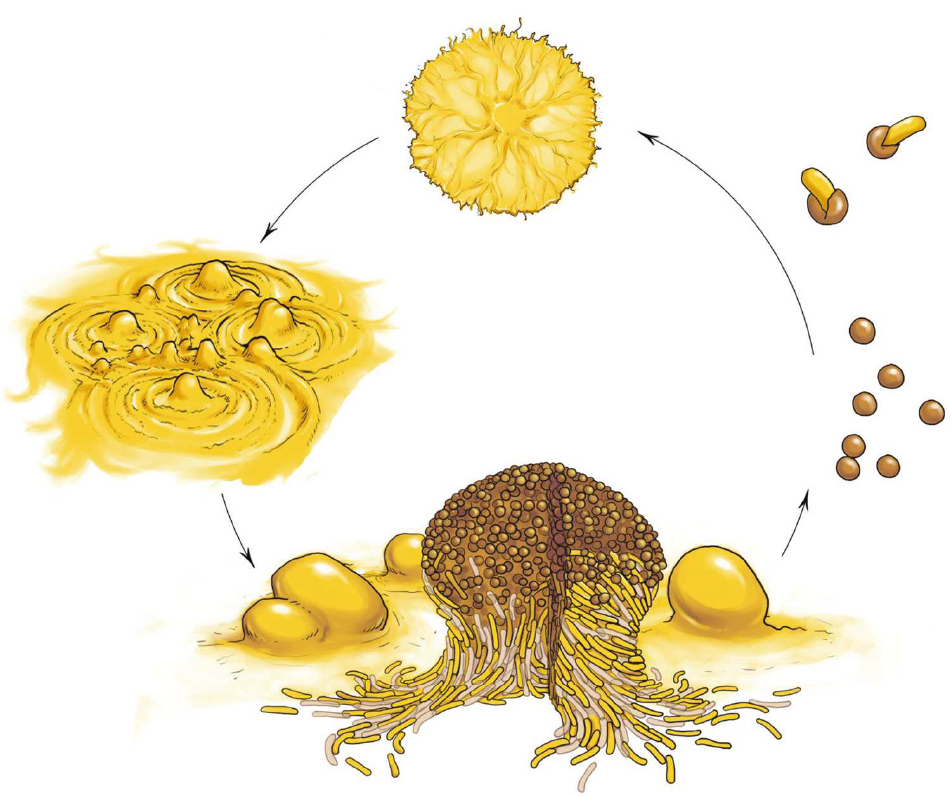
\includegraphics[height=0.85\paperheight]{media/myxo-life}};
\end{tikzpicture}
}
\begin{frame}{The life cycle of Myxo}

\tikz[overlay,remember picture,
shift=(current page.center),
every node/.style={fill=none,text=black}]{
\node at (-2,3) {Swarming};
\node at (-6,0.8){Aggregation};
\node at (-5,-2.8){Fruiting bodies};
\node at (5.3,-1.2){Sporulation};
\node at (5.1,1.9){Germination};
}%
\pause
\tikz[overlay,remember picture,
shift=(current page.center),
every node/.style={fill=none,text=black}]{
\draw[->,line width=6,red] (-1,2.5) .. controls +(-0.6,-0.4) .. (-2.1,1.5);
}%

\footnotetextrelaxed{\fullcite{munoz2016myxobacteria}}
\note{[1:00]
\textit{M.\ xanthus} is a soil bacterium that lives and hunts in groups. While nutrients last, the cells glide together over the substrate as a swarm, a thin film that feeds on prey bacteria.

When the nutrients run out, the swarm aggregates into mounds, and these grow into fruiting bodies of $10^5$ to $10^6$ cells, in which some cells become spores.

\clk A fruiting body is built by stacking layers of cells, so its first step is a second layer on top of the monolayer, the red arrow. My question today is how this first new layer forms.}
\end{frame}
}


\begin{frame}[t]
\begin{wide}{10pt}

\begin{minipage}{0.35\linewidth}
\vspace{1cm}
\centering
\includegraphics<1>[width=0.95\linewidth]{media/fruitingbody/img000}%
\only<2->{%
\animategraphics[autoplay,loop,width=0.95\linewidth,timeline=media/fruitingbody/timeline.txt]{15}{media/fruitingbody/img}{000}{152}}
\end{minipage}%
\hfill
\begin{minipage}{0.64\linewidth}
\alt<3->{
\animategraphics[autoplay,loop,width=\linewidth]{30}{media/colony/img}{00}{95}
}{\phantom{\animategraphics[draft,autoplay,loop,width=\linewidth]{30}{media/colony/img}{00}{95}}
}
\end{minipage}
\end{wide}
\footnotetextrelaxed{(left) \fullcite{curtis2007spatial}}
\footnotetextrelaxed{\onslide<3->{(right)\fullcite{copenhagen}}}
\vspace{-2cm}
\note{[1:00]
On the left, a fruiting body forming under starvation, from Curtis et al. \clk Under starvation it develops so fast that the first new layer is hard to follow.

\clk On the right, a colony on a nutrient-rich substrate, from Copenhagen et al. Here no fruiting bodies form, but new layers and holes still appear throughout the colony. Because the colony stays a thin sheet, single layer-formation events can be tracked, and we expect the same layering mechanism to act under starvation.}
\end{frame}


\begin{frame}{Probability of Layer Formation}
\vspace{-1cm}
\begin{wide}{10pt}
\begin{minipage}{0.6\linewidth}
\vspace{1cm}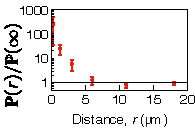
\includegraphics[width=0.8\linewidth]{media/prob_experiment}

\vspace{-3ex}\hfill
\alt<2>{\includegraphics[page=2,width=2cm,trim={0 0 3cm 0},clip]{media/defect-ilustration.pdf}}
{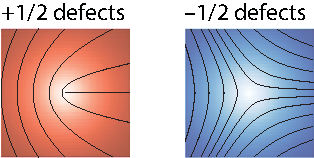
\includegraphics[page=1,width=2cm,trim={0 0 3cm 0},clip]{media/defect-ilustration.pdf}}

\end{minipage}%
\hfill%
\begin{minipage}{0.3\linewidth}
\animategraphics[autoplay,loop,width=0.8\linewidth]{15}{media/defect1/defect1_}{00}{68}

\vspace{1ex}
\animategraphics[autoplay,loop,width=0.8\linewidth]{15}{media/defect2/defect2_}{00}{68}
\end{minipage}

\end{wide}
\footnotetextrelaxed{\fullcite{copenhagen}}
\note{[1:00]
The cells are rods that reverse their direction of motion every few minutes, and neighbouring rods interact in the same way whichever end leads. At long times the monolayer is therefore an active nematic. Its director has topological defects of half-integer charge: the comet-shaped $+1/2$ defect and the three-armed $-1/2$ defect.

Copenhagen et al.\ measured where new layers form relative to $+1/2$ defects: the distribution of distances between new layers and defects, normalized by the same distribution for random points. Near the core, layers form about 200 times more often than far away.

\clk In the movies, the comet marks the $+1/2$ defect: the dot is the core, the bar points to the tail. The new layer appears right next to it.}
\end{frame}


\begin{frame}{\large Large fluctuations \\ in the system}
    \vspace{-9ex}
\begin{wide}{5pt}
    \hfill 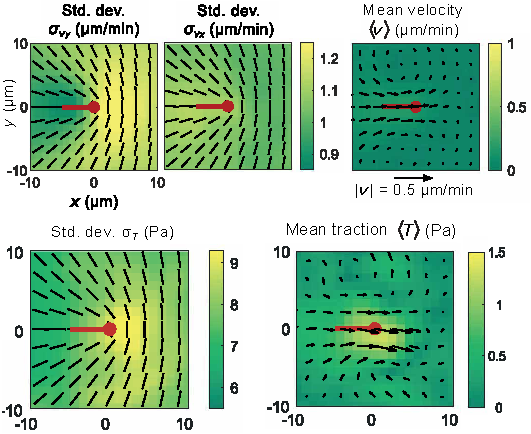
\includegraphics[width=0.65\linewidth]{media/experiment-slide}

\end{wide}

{\footnotesize \fullcite{preprint}}
\note{[0:50]
Why should layers form at defects? Han et al.\ measured the flow and the traction around defects. The mean fields are small: the mean velocity is a fraction of a micrometer per minute, and the mean traction is around one pascal.

The fluctuations, in contrast, are large. The standard deviations of the velocity and of the traction exceed their means everywhere, and the traction fluctuates about ten times more than its mean.}
\end{frame}


\begin{frame}[t]{\large Traction force measurement}
\footnotetextrelaxed{\fullcite{preprint}}

\includegraphics<1>[page=4,width=\linewidth]{media/layer_formation}%
\includegraphics<2>[page=5,width=\linewidth]{media/layer_formation}%
\includegraphics<3-4>[page=6,width=\linewidth]{media/layer_formation}%
\vspace{-2.3ex}
\center{
\onslide<2->{\color[RGB]{180,0,0} Fluorescent beads}%\hspace{1cm}
\hfill
\onslide<3->{\color[RGB]{0,150,0} Traction Force}
}

\onslide<4->{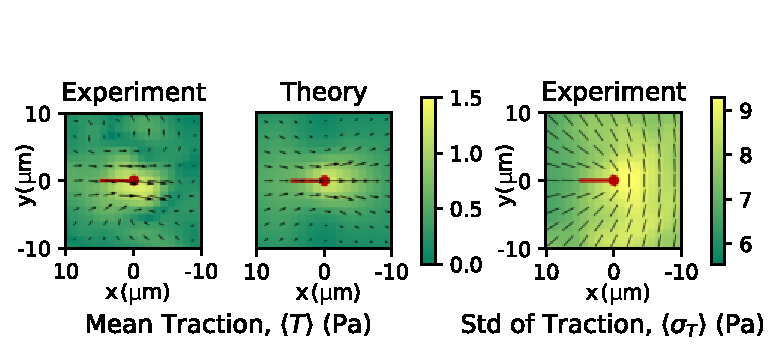
\includegraphics[width=0.9\linewidth,trim={0 0 0 1cm},clip]{media/traction}}
\vspace{-10ex}
\note{[0:50]
The traction is measured on a soft substrate under the cells. \clk Fluorescent beads in the substrate move as the cells pull on it, \clk and their displacements give the traction force.

\clk Around a $+1/2$ defect the mean traction, on the left, is reproduced by a mean-field theory, in the middle. Its standard deviation, on the right, is several times larger, and it stays large in aligned regions away from the defect, where the mean traction nearly vanishes.}
\end{frame}


\begin{frame}[t]{\large Polarity measurement}
\vspace{-3ex}
\begin{wide}{10pt}
\centering
\begin{minipage}{0.3\linewidth}
    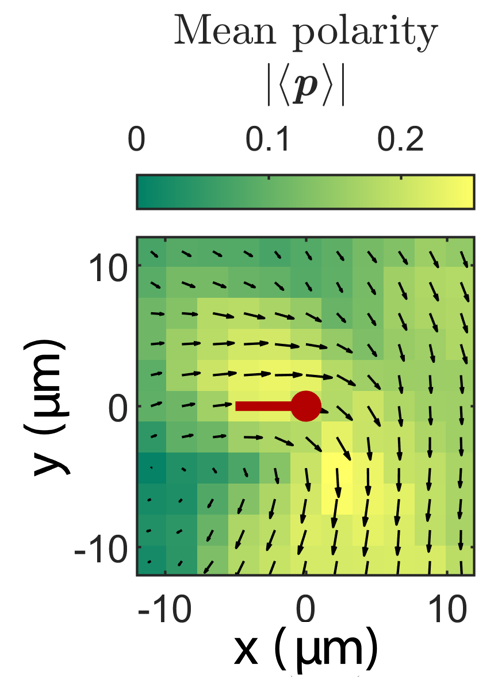
\includegraphics[width=0.9\linewidth]{media/polarity-mean}
\end{minipage}%
\begin{minipage}{0.3\linewidth}
    {\footnotesize ~~~~~~Std. dev. of polarity}

    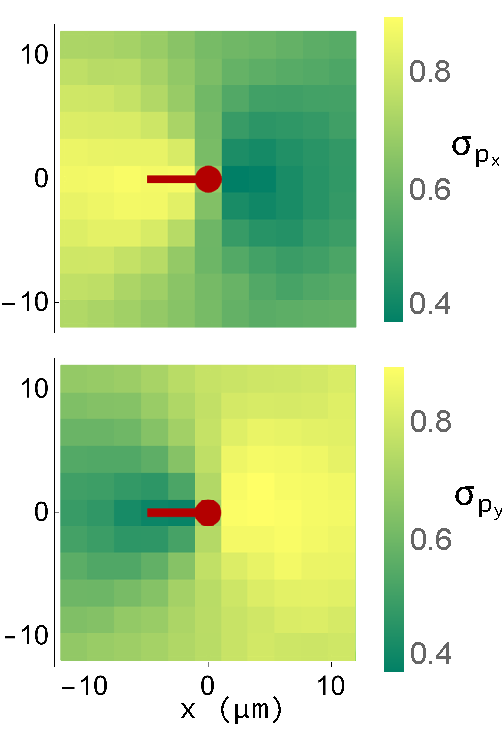
\includegraphics[height=0.85\paperheight]{media/experiment-p-fluctuations}
\end{minipage}~~%
\begin{minipage}{0.3\linewidth}
    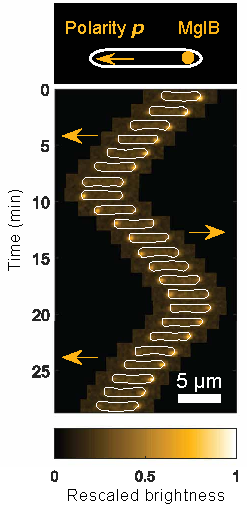
\includegraphics[height=0.9\paperheight]{media/polarity measurement}
\end{minipage}%
\end{wide}
\vspace{-10ex}
\footnotetextrelaxed{\fullcite{preprint}}
\note{[0:50]
Han et al.\ attributed these fluctuations to the local polar order of the cells. On the right, a cell carries a fluorescent polarity marker that switches poles at each reversal.

Around a defect the mean polarity is small, below 0.2, whereas its standard deviation is 0.4 to 0.8. They proposed that these fluctuating polar forces build up local pressure that can trigger new layers, and that active nematic theory, which explains the mean flows, must be extended to capture these fluctuations. This talk is such an extension.}
\end{frame}


\begin{frame}{Outline}
\onslide<+->
\begin{wide}{10pt}
\begin{minipage}[t]{0.5\linewidth}

    \vspace{1cm}
    \begin{itemize}
    \setlength\itemsep{3ex}

    \item average fields are not strong enough for layer formation
    \item Fluctuations in the system are large
    \item \textbf{  \color{bblue}Hypothesis:} fluctuations drive \\ \hfill layer formation.~~~~
\end{itemize}
\end{minipage}%
\hfill\onslide<+->
\begin{minipage}[t]{0.5\linewidth}

{\centering

\vspace{1cm}Polarity fluctuations

\vspace{0.5cm}
$\big\downarrow$

\vspace{0.5cm}
Pressure fluctuations

\vspace{0.5cm}
$\big\downarrow$

\vspace{0.5cm}
{\color<+->{darkgreen}
\textbf<.->{Nucleation Theory}}

\vspace{1cm}
}

\end{minipage}
\end{wide}
\note{[0:40]
So the average fields are too weak to make layers, as I will show in a moment, whereas the fluctuations are large. Our hypothesis is that fluctuations drive layer formation.

\clk The chain is: polarity fluctuations of the cells produce pressure fluctuations, \clk and nucleation theory turns the pressure into a probability of forming a layer. I start with the last step.}
\end{frame}


\begin{frame}[t]{Energetics of Layer Formation}\onslide<+->
\includegraphics<1>[page=1,width=\linewidth]{media/layer_formation}%
\includegraphics<2-4>[page=2,width=\linewidth]{media/layer_formation}%
\only<5>{\animategraphics[autoplay,width=\linewidth]{10}{media/layer_formation_anim}{0}{8}}%
\includegraphics<6->[page=9,width=\linewidth]{media/layer_formation_anim}%
\onslide<+->
\onslide<+->
\vspace{1ex}

\begin{wide}{10pt}
\begin{minipage}{0.5\linewidth}
\begin{itemize}
    \item detach from substrate: $\color{Darkred} W_{cs} A$,
    \item detach from neighbours: $\color{Darkred} W_{cc} h\;\ell$,
    \item surface tension of water: $\color{Darkred} \gamma_w h\;\ell$,
\end{itemize}
\end{minipage}%
\begin{minipage}{0.5\linewidth}
\temporal<.-.(2)>{}{\centering $\ell$ is perimeter}{
\begin{itemize}
    \item adhere to bottom cells: $\color{bblue}-W_{cc} A$,
    \item release pressure: $\color{bblue}-E_p$.
\end{itemize}
}
\end{minipage}

\only<.(1)-.(3)>{\center{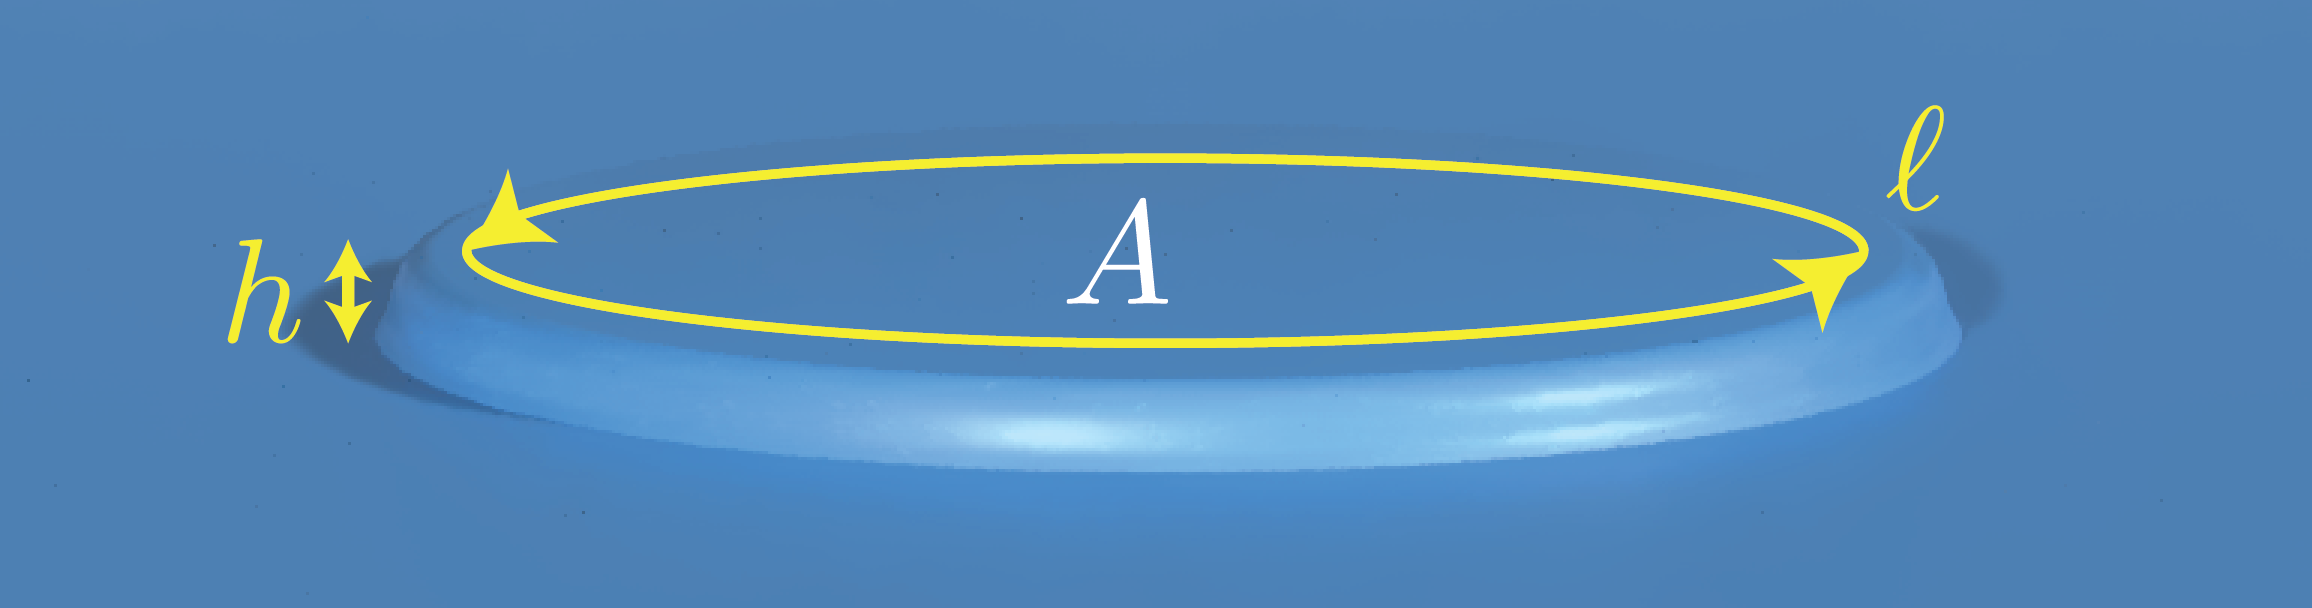
\includegraphics[width=0.8\textwidth]{media/layer_formation_3d_png}}}
\onslide<+(2)->\vspace{0ex}
\vspace{1ex}
\onslide<+->\onslide<+->\onslide<+->

\begin{equation}
    \Delta E={\color{Darkred}W_{cs} A+W_{cc} h\;\ell+\gamma_w h\;\ell}{\color{bblue} -W_{cc} A - E_p}
\end{equation}
\onslide<+->
\vspace{-0.8cm}
\begin{align}
    \onslide<+->{A=\pi (\ell/2)^2 \approx \ell^2} \qquad\qquad E_p(A,\,p) \approx p\;hA
\end{align}
\onslide<+->
\vspace{-1em}
\begin{equation}
\Delta E({\color{darkgreen} A},\,p)=(W_{cs}-W_{cc}) {\color{darkgreen} A} + (W_c+\gamma_w) h\;\sqrt{{\color{darkgreen} A}}- E_p({\color{darkgreen} A},\,p)
\end{equation}
\end{wide}
\note{[1:30]
To connect the pressure with layers we treat layer formation as nucleation. Suppose a patch of cells of area $A$ and perimeter $\ell$ leaves the monolayer.

\clk It pays three costs: it detaches from the substrate, it detaches from its neighbours on the side faces, and it stretches the surface of the water film that wets the colony over its edge.

\clk It gains two things: the adhesion to the cells beneath it, and the elastic energy that the compressed bottom layer releases when it relaxes into the space the patch left, the pressure times the volume $hA$.

\clk Adding up, the energy cost of a new layer has an area term and a perimeter term.}
\end{frame}


\begin{frame}{Energy Barrier}
\vspace{-0.5cm}
\begin{equation}
{\color{bblue}\Delta E(A,\,p)}=(W_{cs}-W_{cc}) A + (W_c+\gamma_w) h\;\sqrt{A}- \overbrace{ p\,hA}^{{\color{darkgreen}E_p(A,\,p)}}
\end{equation}
\bigskip

\hfill
\includegraphics<1>[height=0.8\paperheight,trim={1.5cm 0cm 0cm 1cm},clip]{media/barier/frames/frame4001}%
\includegraphics<2>[height=0.8\paperheight,trim={1.5cm 0cm 0cm 1cm},clip]{media/barier/frames/frame4002}%
\includegraphics<3->[height=0.8\paperheight,trim={1.5cm 0cm 0cm 1cm},clip]{media/barier/frames/frame4003}%
\hspace{1cm}
\note{[1:00]
The perimeter term grows as $\sqrt A$ and the area term as $A$, so at high enough pressure $\Delta E$ rises, reaches a maximum and falls: the barrier of classical nucleation theory, with its maximum at the critical nucleus $A^*$.

\clk Thermal energy is negligible against the adhesion of even one cell, and nothing lifts a group of cells off the substrate together. A new layer must therefore start from a single cell, as seen in the experiments.

\clk If the critical nucleus is smaller than one cell, growth from that cell is downhill. Setting $A^*=A_\text{cell}$ defines a critical pressure $p_\text{crit}$, set by adhesion, the surface tension of water and the cell size. It does not depend on position.}
\end{frame}

\begin{frame}{Barrier Fluctuations}
\hfill
\animategraphics[autoplay,loop,height=0.85\paperheight]{80}{media/barier/frames/frame}{000}{079}
\hspace{1cm}
\note{[0:40]
In classical nucleation theory, fluctuations move the patch along a fixed barrier. Here the pressure itself fluctuates, so the barrier moves up and down with it. Whenever the pressure exceeds $p_\text{crit}$, the barrier at one cell is gone and a cell can leave the monolayer.}
\end{frame}


\begin{frame}
\begin{wide}{10pt}
\vspace{0.5ex}
\onslide<+->
\begin{minipage}[t]{0.47\linewidth}
\centerline{ {\color<2->{litelitegray}Average} pressure around $+\tfrac{1}{2}$ defect}
\includegraphics<1>[width=1.\linewidth]{media/pressure-on-defect}%
\only<2->{\animategraphics[autoplay,loop,width=1\linewidth]{5}{media/pressure-frames/frame}{1}{5}}
\end{minipage}%
\begin{minipage}[t]{0.5\linewidth}
\onslide<+->
$$p(\r) =\la p(\r) \ra + {\color{purple} \delta p(\r)} \onslide<.(1)->{\color{darkred} \quad> p_c}$$
$${\color{purple} \delta p(\r)} \sim \mathhlbox<5->{litegreen}{\mathcal{N}(0,\sigma_p(\r)^2)}$$
\end{minipage}
\vspace{-5.8ex}
\onslide<+->\onslide<+->

\hfill\onslide<.(1)->{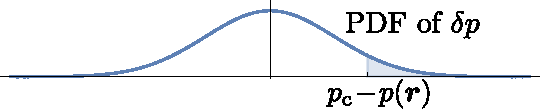
\includegraphics[width=0.65\linewidth]{media/normal_tail}}
\vspace{-0.2cm}
$$\mathbb{P}\left(\text{New layer} \atop\text{at point }{\r}\right)=\mathbb{P}\Big({\color{purple} \delta p} > {\color{darkred} p_c}-\la p(\r) \ra\!\Big)
\onslide<+->
\onslide<+->
=1-\text{Erf}\left(\frac{{\color{darkred} p_c}-\la p(\r)\ra}{\sigma_p(\r)}\right)$$
\vspace{-2ex}
\end{wide}
\note{[1:30]
The average pressure around a $+1/2$ defect, on the left, is of the order of the active stress, three to four orders of magnitude below $p_\text{crit}$. On average, no layer would ever form.

\clk So we write the pressure as its mean plus a fluctuation, and a layer can form where the fluctuation exceeds $p_\text{crit}$ minus the mean.

\clk If the fluctuation is Gaussian with standard deviation $\sigma_p$, the probability of a new layer at $\r$ is a Gaussian tail, \clk one minus an error function.

Everything therefore reduces to the standard deviation of the pressure around a defect, and that is set by the noise in the system.}
\end{frame}


\begin{frame}[t]
\begin{minipage}{0.6\linewidth}

\end{minipage}%
\hfill%
\begin{minipage}{0.4\linewidth}
{\Large \color{bblue} ~~Outline}

{\centering

\vspace{1cm}

\alt<2->{{{\color{bblue}Microscopic model}}}{{\color{darkred}Polarity fluctuations}}


\vspace{0.5cm}
$\big\downarrow$

\vspace{0.5cm}
{\color{darkred}Pressure fluctuations}

\vspace{0.5cm}
$\big\downarrow$

\vspace{0.5cm}
{\color{darkgreen}Nucleation Theory {\Large \checkmark}}

\vspace{1cm}
}
\end{minipage}%
\note{[0:20]
Nucleation theory is in place. What remains is to get the pressure fluctuations from the polarity fluctuations of the cells, \clk and for that we start from a microscopic model of the cells.}
\end{frame}


% ===========================================================================
% Part 1: the microscopic model and Dean's equation
% ===========================================================================
\begin{frame}{Microscopic model of reversing bacteria}
\onslide<+->
\begin{wide}{30pt}
\begin{minipage}[c]{0.4\linewidth}
    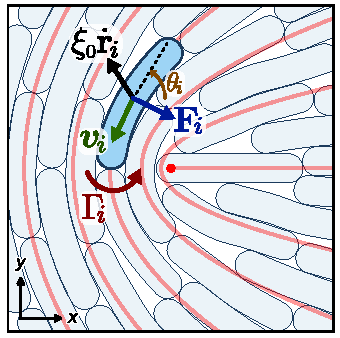
\includegraphics[width=\linewidth,page=1]{media/paper-main}
\end{minipage}%
\begin{minipage}[c]{0.6\linewidth}
    \small\setlength{\abovedisplayskip}{3pt}\setlength{\belowdisplayskip}{3pt}
    \begin{align*}
        \frac{\d\r_i}{\d t} &= \colI{\frac{\rho_0}{\xi_0}\F_i} + \colA{v_0\,\p(\theta_i)\, k_i}
        \\
        \frac{\d\theta_i}{\d t} &= \colI{\frac{\rho_0}{\xir}\Gamma_i} + \colR{\lambda_i}
        \\[1ex]
        \onslide<2->{\colA{\la k_i(t)k_j(t')\ra}} &\onslide<2->{= \delta_{ij}\,\ee^{-2\frev|t-t'|}}
        \\
        \onslide<2->{\colR{\la\lambda_i(t)\lambda_j(t')\ra}} &\onslide<2->{= 2\Lambda\,\delta_{ij}\,\delta(t-t')}
        \\[1ex]
        \onslide<3->{\colI{\F_i}} &\onslide<3->{= -\pd{}{\r}\textstyle\sum_{j} V(\r_i-\r_j,\theta_i,\theta_j)}
        \\
        \onslide<3->{\colI{\Gamma_i}} &\onslide<3->{= -\pd{}{\theta}\textstyle\sum_{j} V(\r_i-\r_j,\theta_i,\theta_j)}
    \end{align*}
    {\footnotesize
    \onslide<2->{reversals: $\colA{k_i=\pm1}$, switching at rate $\frev$}

    \onslide<4->{$V(\r-\r',\theta,\theta')=V(\r'-\r,\theta',\theta)$ $\Rightarrow$ no self force}}
\end{minipage}

\end{wide}
\vspace{2ex}
\onslide<1->
\modellegend
\note{[1:20]
We start from the cells. Each cell is an overdamped rod with position $\r_i$ and orientation $\theta_i$: friction with the substrate balances the forces, so the velocity is proportional to the force. A rod moves for two reasons: the force of its neighbours, in blue, and self-propulsion at speed $v_0$ along its own axis, in red. Its orientation changes by the torque of the neighbours and by rotational noise, in green.

\clk The sign $k_i$ flips at each reversal, at rate $f_\text{rev}$. It is a random telegraph signal with correlation time $1/(2f_\text{rev})$.

\clk Force and torque come from a pair potential $V$, which we never need explicitly. \clk Because the potential is symmetric between two rods, a rod exerts no force on itself.}
\end{frame}


\begin{frame}[t,label=m-dean]{Dean's equation: Langevin equation for the density}
\small\setlength{\abovedisplayskip}{2pt}\setlength{\belowdisplayskip}{2pt}
\onslide<+->
\begin{columns}[c,totalwidth=\textwidth]
\column{0.38\textwidth}
\centering
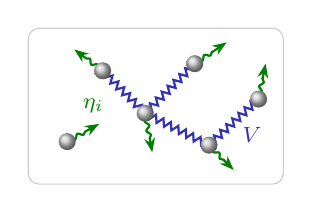
\begin{tikzpicture}[x=0.9cm,y=0.9cm]
  \draw[litelitegray,rounded corners] (-0.3,-0.25) rectangle (3.3,1.95);
  \coordinate (P1) at (0.25,0.35); \coordinate (P2) at (0.75,1.35);
  \coordinate (P3) at (1.35,0.75); \coordinate (P4) at (2.05,1.45);
  \coordinate (P5) at (2.25,0.30); \coordinate (P6) at (2.95,0.95);
  \foreach \a/\b in {P2/P3,P3/P4,P3/P5,P5/P6}
    \draw[bblue,thick,decorate,decoration={zigzag,amplitude=1.3pt,segment length=3pt}] (\a) -- (\b);
  \foreach \p/\dx/\dy in {P1/0.45/0.25,P2/-0.4/0.3,P3/0.1/-0.55,P4/0.45/0.3,P5/0.35/-0.35,P6/0.1/0.5}
    \draw[darkgreen,thick,-{Stealth[length=1.8mm]},decorate,
          decoration={snake,amplitude=0.7pt,segment length=3.5pt,post length=1.8mm}] (\p) -- ++(\dx,\dy);
  \foreach \p in {P1,P2,P3,P4,P5,P6} \shade[ball color=gray!45] (\p) circle (0.12);
  \node[font=\footnotesize,text=bblue,anchor=north west,inner sep=1pt] at (2.68,0.6) {$V$};
  \node[font=\footnotesize,text=darkgreen,anchor=south] at (0.62,0.62) {$\eta_i$};
\end{tikzpicture}\\[1ex]
$\displaystyle\frac{\d X_i}{\d t} = \colN{\eta_i(t)} - \colI{\textstyle\sum_{j}\nabla V(X_i-X_j)}$\\[0.5ex]
{\footnotesize $N$ Brownian particles at temperature $T$}
\column{0.06\textwidth}
\centering{\LARGE $\Rightarrow$}
\column{0.56\textwidth}
\centering
density $\rho(x,t)=\sum_i\delta\big(x-X_i(t)\big)$ obeys \textbf{exactly}
\[\boxed{\partial_t\rho=\nabla\cdot\Big(\rho\,\nabla\frac{\delta F}{\delta\rho}\Big)+\colN{\nabla\cdot\big(\eta\,\sqrt{\rho}\,\big)}}\]
\[F[\rho]=\colI{\frac12\!\int\!\d x\,\d y\;\rho(x)\,V(x-y)\,\rho(y)}+\colD{T\!\!\int\!\d x\;\rho\log\rho}\]
{\footnotesize $\colN{\la\eta^\mu(x,t)\,\eta^\nu(y,t')\ra}=2T\,\delta^{\mu\nu}\,\delta(x-y)\,\delta(t-t')$}
\end{columns}

\vspace{1.5ex}
\onslide<+->
\begin{columns}[T,totalwidth=\textwidth]
\column{0.32\textwidth}\centering\textbf{exact}\\{\footnotesize any $N$, any pair potential $V$}
\column{0.32\textwidth}\centering\textbf{$N$ conserved}\\{\footnotesize in every realization}
\column{0.32\textwidth}\centering\colN{\textbf{multiplicative noise}}\\{\footnotesize no particles $\Rightarrow$ no fluctuations}
\end{columns}

\vspace{1.5ex}
\onslide<+->
\centering
\msg{\footnotesize Equilibrium: the fluctuation--dissipation theorem fixes the noise.\quad
Active matter: it does not, and the noise is usually added by hand.\\[0.2ex]
\small\textbf{Dean: the noise follows from the dynamics of the particles.}}

\onslide<1->
\footnotetextrelaxed{\fullcite{dean1996}}
\note{[2:00]
To get the pressure fluctuations we need field equations that keep the noise of the single cells. The tool for that is Dean's equation.

Take $N$ Brownian particles at temperature $T$, each kicked by its own noise and interacting through a pair potential. Dean showed in 1996 that their density, written as a sum of delta functions, obeys exactly a closed stochastic equation. The deterministic part is the familiar gradient flow of a free energy, with the interactions and the ideal-gas entropy. The noise, in green, is a random current whose amplitude is the square root of the density.

\clk Three properties come for free. The equation is exact, for any number of particles and any potential. Every term is a divergence, so the number of particles is conserved in every realization. And the noise is multiplicative: where there are no particles, the density cannot fluctuate.

\clk For us the important point is the box. In equilibrium the fluctuation--dissipation theorem fixes the noise from the friction. In active matter it does not, so continuum theories usually add noise by hand, with a free amplitude. Dean's route derives the noise from the motion of the particles, and we need exactly that, because the layering probability depends exponentially on this amplitude.}
\end{frame}


\begin{frame}[t,label=m-caveats]{Caveats: what is $\rho$ in Dean's equation?}
\onslide<+->
\centering
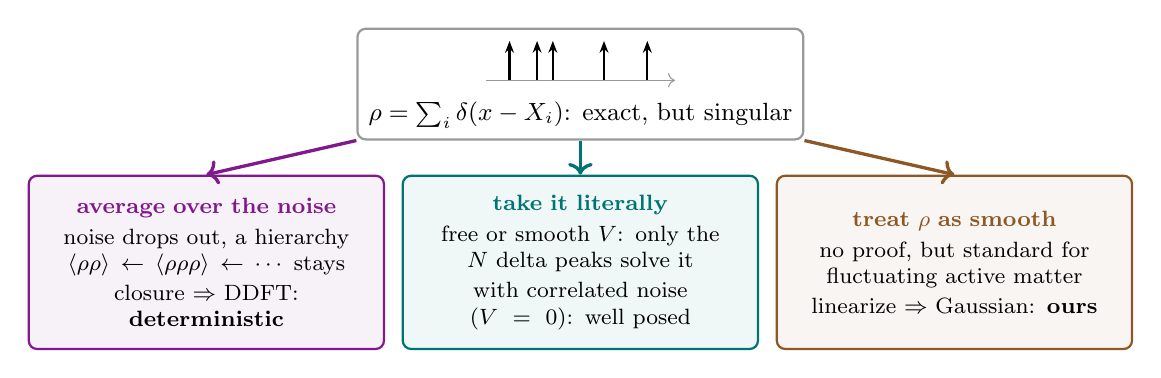
\begin{tikzpicture}
  \node[draw=litegray,thick,rounded corners=3pt,inner sep=4pt,align=center,font=\small] (rho) at (0,0) {%
    \tikz[x=1cm,y=1cm]{\draw[->,litegray] (0,0) -- (2.4,0);
      \foreach \s in {0.3,0.65,0.85,1.5,2.05}{\draw[-{Stealth[length=1.5mm]},thick] (\s,0) -- (\s,0.5);}}\\[1pt]
    $\rho=\sum_i\delta(x-X_i)$: exact, but singular};
  \node[rhobox=laneD,visible on=<2->] (avg) at (-4.75,-1.15) {%
    {\color{laneD}\textbf{average over the noise}}\\[0.5ex]
    noise drops out, a hierarchy\\ $\la\rho\rho\ra\leftarrow\la\rho\rho\rho\ra\leftarrow\cdots$ stays\\[0.4ex]
    closure $\Rightarrow$ DDFT: \textbf{deterministic}};
  \node[rhobox=laneM,visible on=<3->] (lit) at (0,-1.15) {%
    {\color{laneM}\textbf{take it literally}}\\[0.5ex]
    free or smooth $V$: only the\\ $N$ delta peaks solve it\\[0.4ex]
    with correlated noise\\ ($V=0$): well posed};
  \node[rhobox=laneS,visible on=<4->] (smo) at (4.75,-1.15) {%
    {\color{laneS}\textbf{treat $\rho$ as smooth}}\\[0.5ex]
    no proof, but standard for\\ fluctuating active matter\\[0.4ex]
    linearize $\Rightarrow$ Gaussian: \textbf{ours}};
  \draw[->,very thick,laneD,visible on=<2->] (rho.south west) -- (avg.north);
  \draw[->,very thick,laneM,visible on=<3->] (rho.south) -- (lit.north);
  \draw[->,very thick,laneS,visible on=<4->] (rho.south east) -- (smo.north);
\end{tikzpicture}

\vspace{1ex}
\onslide<+->
\msg[0.97]{\footnotesize\raggedright
\textbf{\small Two caveats for our rods}\\[0.2ex]
1.\ It\^o calculus needs white noise: the reversals (correlation time $1/(2\frev)\approx5$~min) are treated as white noise.\\
2.\ The Gaussian continuum is used down to one cell width, where a cell-width square holds $\approx0.06$ cells.}
\note{[1:45]
What does $\rho$ mean in Dean's equation? It is exact, but it is a sum of delta functions, which is singular. There are three ways to live with that.

\clk Average over the noise: the noise drops out, but the equation for the mean density contains the pair correlation, that one the three-point correlation, and so on. Closing this hierarchy gives dynamical density functional theory, which is deterministic, so it loses the fluctuations we want.

\clk Take the equation literally: for free particles or smooth potentials, Konarovskyi and co-workers proved that its only solutions are the $N$ delta peaks themselves, so nothing is gained. For free particles with spatially correlated noise, read in the Stratonovich sense, Fehrman and Gess showed that it is well posed.

\clk Treat $\rho$ as a smooth field. There is no rigorous proof, but this is what the fluctuating theories of active particles do, from Tailleur and Cates to Bertin et al. We do it too, and we then linearize around a steady state, which makes the fluctuations Gaussian.

\clk For our cells two caveats matter. Dean's derivation needs white noise, so we treat the reversals as white noise, although their correlation time is about five minutes. And we use the continuum, with Gaussian statistics, down to the width of one cell, where a cell-width square holds on average only about 0.06 cells. I come back to both at the end.}
\end{frame}


\begin{frame}[t,label=m-dean-rods]{Dean's equation for reversing rods}
\small\setlength{\abovedisplayskip}{3pt}\setlength{\belowdisplayskip}{3pt}
\begin{wide}{10pt}
\onslide<+->
Reversals as white noise, for times $\gg1/(2\frev)$:\quad
$\colA{\la k_i(t)k_j(t')\ra}=\delta_{ij}\,\ee^{-2\frev|t-t'|}\approx\frev^{-1}\,\delta_{ij}\,\delta(t-t')$

\vspace{1ex}
\onslide<+->
Joint density:\quad $\varrho_t(\r,\theta)=\rho_0^{-1}\sum_i\delta\big(\r-\r_i(t)\big)\,\delta\big(\theta-\theta_i(t)\big)$

\vspace{1ex}
\onslide<+->
Same steps as Dean, now over $(\r,\theta)$, exact in the white-noise limit:
\begin{equation*}
    \begin{aligned}
    \partial_t\varrho_t = {}&
    \lab{\colI{\frac1{\xi_0}\pd{}{\r}\tcdot\left(\varrho_t\pd{}{\r}\frac{\delta\calF}{\delta\varrho}\right)}}{translational friction}
    + \lab{\colI{\frac1{\xir}\pd{}{\theta}\!\left(\varrho_t\pd{}{\theta}\frac{\delta\calF}{\delta\varrho}\right)}}{rotational friction}
    + \lab{\colA{\frac{v_0^2}{2\frev}\,p_\alpha p_\beta\,\pd{^2\varrho_t}{r_\alpha\partial r_\beta}}}{It\^o term}
    + \lab{\colR{\Lambda\,\pd{^2\varrho_t}{\theta^2}}}{rot.\ diffusion}
    \\
    &\colA{- \pd{}{\r}\tcdot\left(\sqrt{\varrho_t}\,\p(\theta)\,k(\r,\theta,t)\right)}
    \colR{- \pd{}{\theta}\!\left(\sqrt{\varrho_t}\,\lambda(\r,\theta,t)\right)}
    \end{aligned}
\end{equation*}
\onslide<+->
\[\colA{\la k\,k'\ra}=\frac{v_0^2}{\frev\,\rho_0}\,\Delta,\qquad
  \colR{\la\lambda\,\lambda'\ra}=\frac{2\Lambda}{\rho_0}\,\Delta,\qquad
  \Delta=\delta(t-t')\,\delta(\r-\r')\,\delta(\theta-\theta')\]
\centering
\msg[0.9]{It\^o term and reversal noise share $\colA{v_0^2/\frev}$: the same reversals drive the mean and the fluctuations}
\end{wide}
\onslide<1->
\vfill
\modellegend
\note{[1:30]
Our rods do not fit Dean's setting directly, because the reversal noise $k_i$ is not white: it is a telegraph signal with correlation time $1/(2f_\text{rev})$. At times long compared with that, we replace it by white noise of the same integrated strength.

\clk Then we follow the joint density of positions and orientations, again a sum of delta functions.

\clk The same steps as Dean's give an exact equation for it. The first two terms are the forces and torques of the neighbours, with translational and rotational friction. The third is the It\^o term of self-propulsion: with reversals, each rod diffuses along its own axis, with diffusivity $v_0^2/(2f_\text{rev})$. The fourth is rotational diffusion. The second line holds the two noises, again with the square root of the density.

\clk The key point is that the It\^o term and the reversal noise carry the same amplitude $v_0^2/f_\text{rev}$, so the same reversals set the mean active stress and the fluctuations.}
\end{frame}


\begin{frame}[t]{Free energy and pressure}
\small\setlength{\abovedisplayskip}{4pt}\setlength{\belowdisplayskip}{4pt}
\onslide<+->
Fields: density $\rho(\r,t)=\int\!\d\theta\,\varrho_t$ \;and nematic tensor $\Q(\r,t)=\int\!\d\theta\,\varrho_t\,\hat\Q(\theta)$, \quad $\hat\Q=2\p\p-\I$

\vspace{1ex}
$V$ unknown $\Rightarrow$ assume $\colI{\calF}$ depends on $\varrho$ only through $\rho$ and $\Q$:
\[\colI{\calF[\varrho]=F[\rho,\Q]}=\int\!\d\r\;\mathfrak f\bigl(\rho,\Q,\partial_\r\Q\bigr)\]
\onslide<+->
\[\mathfrak f = \lab{\frac B2(\rho-1)^2}{compression, bulk modulus $B$}
  + \lab{\frac a2(\Q\!:\!\Q)+\frac b4(\Q\!:\!\Q)^2}{Landau--de Gennes, $a<0$: order}
  + \lab{\frac K2(\partial_\r\Q)\!:\!(\partial_\r\Q)}{elasticity}\]
\onslide<+->
\vspace{1ex}
Pressure from the compression term:
\[\boxed{p=\tfrac B2\left(\rho^2-1\right)\simeq B(\rho-1)}\]
\centering
{\footnotesize two-dimensional pressure (force per length);\; $B$ turns density fluctuations into pressure fluctuations}
\note{[0:50]
We do not know the pair potential between two cells, so we do not compute the free energy from it. Instead we assume that it depends on the rods only through the density $\rho$ and the nematic tensor $\Q$, the two lowest angular moments.

\clk We take the simplest choice: a compression term with bulk modulus $B$, which keeps the monolayer nearly incompressible, and the standard Landau--de Gennes free energy of a nematic, with one elastic constant $K$.

\clk The pressure follows from the compression term alone, $p\simeq B(\rho-1)$. So $B$, the stiffness of the monolayer against compression, converts density fluctuations into pressure fluctuations. This pressure is two-dimensional, a force per unit length of the monolayer.}
\end{frame}


\begin{frame}[t,label=m-density]{Density equation: one coefficient for force and noise}
\small\setlength{\abovedisplayskip}{3pt}\setlength{\belowdisplayskip}{3pt}
\onslide<+->
Integrate over $\theta$, leading order in $1/B$:
\[\partial_t\rho=-\nabla\cdot\Big[\frac1{\xi_0}\big(\lab{\colI{-B\nabla\rho}}{pressure}+\lab{\colI{\Q\!:\!\nabla\H}}{elastic}+\lab{\colA{\fa}}{active}\big)+\lab{\colA{\bEta_\rho}}{noise}\Big]\]
\onslide<+->
\[\colA{f^\mathrm{a}_\alpha}=-\colA{\zeta}\,\partial_\beta Q_\ab,\qquad \boxed{\colA{\zeta=\frac{\xi_0v_0^2}{4\frev}}}
  \qquad{\footnotesize\text{extensile active stress, largest at a defect core}}\]
\onslide<+->
\[\colA{\la\eta^\rho_\alpha(\r,t)\,\eta^\rho_\beta(\r',t')\ra}=\frac{2\colA{\zeta}}{\xi_0\rho_0}\big[Q_\ab+\rho\,\delta_\ab\big]\,\delta(\r-\r')\,\delta(t-t')\]
\centering
{\footnotesize same $\colA{\zeta}$: faster reversals $\Rightarrow$ weaker active stress \emph{and} weaker noise;\quad noise stronger along the rods}

\vspace{1.5ex}
\onslide<+->
\msg[0.97]{\raggedright
Polarity view: $\bs P=\rho_0^{-1}\sum_ik_i\,\p(\theta_i)\,\delta(\r-\r_i)$, relaxed by reversals at rate $2\frev$:\\[0.5ex]
\centering
$\colA{\fa=\xi_0v_0\,\bs P_Q}$,\quad $\bs P_Q=-\dfrac{v_0}{4\frev}\nabla\cdot\Q$ \;(splay and bend)\qquad
$\colA{\bEta_\rho=v_0\,\big(\bs P-\la\bs P\ra\big)}$}
\note{[1:30]
Integrating over orientations gives a continuity equation for the density. The flux has a passive part, the pressure gradient and an elastic force from the nematic field, and an active part.

\clk The active force is minus $\zeta$ times the divergence of $\Q$, the force of an extensile active stress. Its coefficient $\zeta=\xi_0v_0^2/(4f_\text{rev})$ comes entirely from self-propulsion and reversals, so a fast-reversing colony is less active. The force vanishes in a uniform nematic and is largest where the director bends fastest, at a defect core.

\clk The last term is the noise of the flux. Its amplitude is set by the same $\zeta$, and it is anisotropic: stronger along the rods than across them, because a cell runs along its own axis.

\clk The same equations follow from a theory that keeps the polarity $\bs P$ of the cells. Splay and bend of the director induce a mean polarity $\bs P_Q$, and the active force is the friction of that polarity. The fluctuation of $\bs P$ around its mean, times $v_0$, is the density noise, so the noise of this equation is the polarity fluctuation that Han et al.\ measured.}
\end{frame}


\begin{frame}[t,label=m-closure]{The closure we have to choose}
\small\setlength{\abovedisplayskip}{3pt}\setlength{\belowdisplayskip}{3pt}
\onslide<+->
Multiply by $\hat\Q(\theta)$, integrate over $\theta$: averages over the rods appear, which $\rho$ and $\Q$ do not fix
\begin{align*}
\partial_t Q_\ab = {}& \colI{\frac1{\xi_0}\partial_\gamma\Bigl(Q_\ab\,\partial_\gamma\frac{\delta F}{\delta\rho}
+ \mathhlbox{liteyellow}{\langle\hat Q_\ab\hat Q_\mn\rangle_\varrho}\,\partial_\gamma\frac{\delta F}{\delta Q_\mn}\Bigr)
- \frac1{\xir}\mathhlbox{liteyellow}{\langle\hat Q'_\ab\hat Q'_\mn\rangle_\varrho}\,\frac{\delta F}{\delta Q_\mn}}
\colR{- 4\Lambda Q_\ab}
\\
&\colA{+ \frac{\zeta}{\xi_0}\bigl(\nabla^2Q_\ab + \partial_\mu\partial_\nu\mathhlbox{liteyellow}{\langle\hat Q_\ab\hat Q_\mn\rangle_\varrho}\bigr)} + \text{noises},
\qquad \la X\ra_\varrho=\textstyle\int\!\d\theta\,\varrho_t\,X(\theta)
\end{align*}
\vspace{0.5ex}
\begin{columns}[T,totalwidth=\textwidth]
\column{0.74\textwidth}
\onslide<+->
Closure: maximum entropy at given $\rho$, $\Q$ $\Rightarrow$ von Mises in $2\theta$\\[0.5ex]
\centering
$\varrho(\theta)=\dfrac{\rho\,\ee^{\kappa\cos2(\theta-\theta_0)}}{2\pi I_0(\kappa)}$,\qquad $I_1(\kappa)/I_0(\kappa)=S$\\[1ex]
\raggedright
\onslide<+->
exact:\quad $\langle\hat\Q\hat\Q\rangle_\varrho=\rho\J+\frac{g_2(S)}{2\rho}\,\U(\Q)$\\[0.3ex]
lowest order:\quad $\mathhlbox{liteyellow}{\langle\hat\Q\hat\Q\rangle_\varrho\simeq\rho\J}$,\quad error $O(S^2)$\\[1ex]
\onslide<+->
{\color{darkred} but $S_0=0.9$ in the monolayer: $g_2=0.82$, not $\tfrac12$}
\column{0.24\textwidth}
\onslide<2->
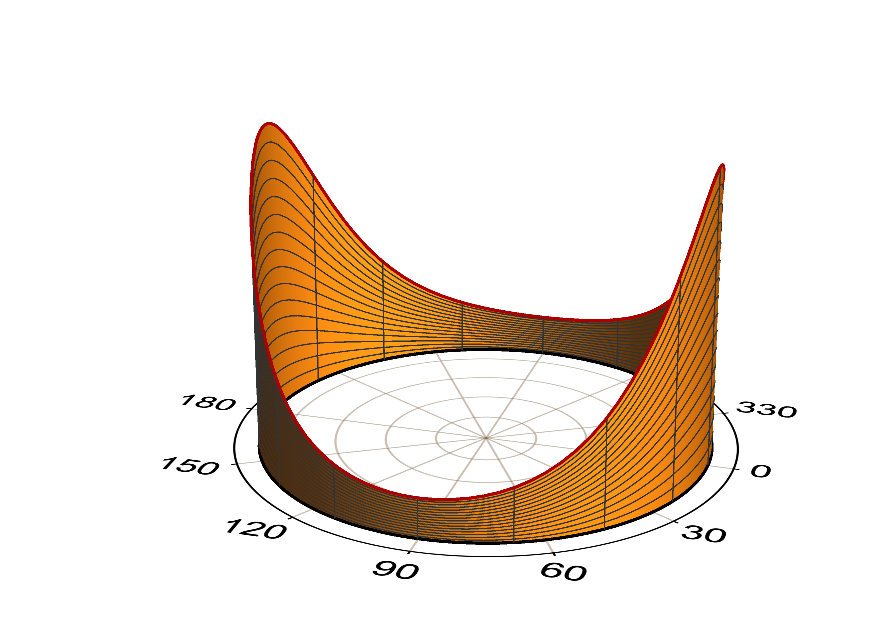
\includegraphics[width=\linewidth,trim={1.5cm 0 1.5cm 1.5cm},clip]{media/pdf-mathematica-2}
\end{columns}
\note{[1:15]
For the nematic tensor we multiply the joint equation by $\hat\Q(\theta)$ and integrate over angles. Now the equation is not closed: averages over the rods like $\la\hat\Q\hat\Q\ra$ appear, highlighted, and $\rho$ and $\Q$ do not fix them.

\clk We close them with the distribution of maximum entropy at given $\rho$ and $\Q$. Because $\Q$ contains only $\cos2\theta$ and $\sin2\theta$, this is a von Mises distribution in $2\theta$, like the picture, with both ends of a rod weighted equally.

\clk Its moments are known exactly, with a coefficient $g_2$ that depends on the order $S$. Expanded to lowest order in $S$ they become simple, $\la\hat\Q\hat\Q\ra\simeq\rho\J$, accurate to order $S^2$. This is what continuum theories derived from particles usually do.

\clk But a monolayer is strongly ordered, $S_0=0.9$, where $g_2$ is 0.82 instead of 1/2. So the closure is not accurate around the defect, and the next slide shows what that costs.}
\end{frame}


\begin{frame}[t,label=m-cost]{What the lowest-order closure costs}
\onslide<+->
At $S_0=0.9$ the lowest-order closure breaks in three places:
\vspace{2ex}
\begin{enumerate}\setlength{\itemsep}{2.5ex}
\item<+-> \textbf{With the elastic force, ill posed for $S>1/\sqrt2$}\\
{\small order perturbations grow as $(K/\xi_0)(2S^2-1)\,k^4$}\\
{\small $\Rightarrow$ \colI{drop the elastic force} on the cells: both $\nabla\H$ terms\\
\color{softgray} usual in dry active nematics, also for \textit{M.\ xanthus}; here forced by the closure}
\item<+-> \textbf{Noise covariance not positive for $S>S_\star=(\sqrt5-1)/2\simeq0.62$}\\
{\small $\Rightarrow$ numerics: noise from the exact von Mises moments\\
\color{softgray} the analytic result needs only the density noise, which is exact}
\item<+-> \textbf{Drift of a $+1/2$ defect in the wrong direction}\hfill{\small $\to$ results}
\end{enumerate}
\note{[1:10]
At the strong order of the monolayer, the lowest-order closure breaks in three places.

\clk First, with the elastic force on the cells, the closed equations become ill posed wherever $S$ exceeds $1/\sqrt2$: perturbations of the order grow faster the shorter their wavelength. We therefore drop the elastic force. Most continuum models of dry active nematics, including those of \textit{M.\ xanthus} monolayers, drop it too, but here the closure forces it.

\clk Second, the noise that the closure gives has a covariance with a negative eigenvalue above $S\approx0.62$, so no noise could have it. In the numerics we therefore build the noise from the exact moments. The analytic result I show later needs only the density noise, which is exact.

\clk Third, and this matters for the experiments: the closure decides in which direction a $+1/2$ defect moves, and it gets it wrong. I come back to this in the results.}
\end{frame}


\begin{frame}[t,label=m-final]{Fluctuating active nematic}
\small\setlength{\abovedisplayskip}{3pt}\setlength{\belowdisplayskip}{3pt}
\onslide<+->
Closed stochastic equations for $\rho$ and $\Q$:
\begin{align*}
    \partial_t\rho ={}& -\nabla\tcdot\Bigl[
    \frac1{\xi_0}\bigl(\colI{-B\nabla\rho} + \alt<2->{{\color{litegray}\Q\!:\!\nabla\H}}{\colI{\Q\!:\!\nabla\H}} + \colA{\fa}\bigr)
    + \colA{\bEta_{\rho}}\Bigr]
    \\
    \partial_t \Q = {}& -\nabla\!\cdot\!\Bigl[\frac1{\xi_0}
    \bigl(\lab{\colI{-\Q B \nabla\rho}}{cross-coupling} + \alt<2->{{\color{litegray}\nabla \H}}{\colI{\nabla \H}}\bigr) + \colA{\bEta^\Q}\Bigr] + \frac4{\xir} \Ha + \colR{\f^Q}
    \\[2ex]
    &\Ha = -a'\Q - b(\Q\!:\!\Q)\Q + K'\nabla^2\Q,
    \qquad a' = \colI{a}+\colR{\Lambda\xir},
    \qquad K' = \colI{K}+\colA{\zeta\xir/(4\xi_0)}
    \\
    &\colA{\fa} = -\colA{\zeta}\,\nabla\cdot\Q,
    \qquad \colA{\zeta = \frac{\xi_0v_0^2}{4\frev}}
\end{align*}
\onslide<+->
\begin{itemize}\setlength{\itemsep}{0.5ex}
    \item elastic force dropped (gray): the pressure is the only passive stress
    \item activity enters three times: $\colA{\fa}$, the noise amplitudes, and $\colA{K'}$
    \item the cross-coupling (pressure-driven flow carries alignment) sets a $+1/2$ defect in motion
\end{itemize}
\onslide<1->
\vfill
\modellegend
\note{[0:50]
These are the equations we solve: a fluctuating active nematic for the density and the nematic tensor.

\clk Without the elastic terms, in gray, the pressure is the only passive stress. Activity enters in three places: the active force, the amplitude of the noises, and the elastic constant $K'$, renormalized because the rods carry their alignment as they run. The cross-coupling in the second equation, the transport of alignment by the pressure-driven flow, is what sets a $+1/2$ defect in motion.}
\end{frame}


% ===========================================================================
% Part 3: results
% ===========================================================================
\begin{frame}[t]
\begin{minipage}{0.55\linewidth}
\vspace{1.2cm}
{\Large\color{bblue} Results}

\vspace{2ex}
\begin{enumerate}\setlength{\itemsep}{1.5ex}
\item parameters
\item steady state of a $+1/2$ defect, and its drift
\item density fluctuations around the defect
\item layer formation
\end{enumerate}
\end{minipage}%
\hfill%
\begin{minipage}{0.4\linewidth}
{\centering

\vspace{1.9cm}
{\color{bblue}Microscopic model {\Large \checkmark}}

\vspace{0.5cm}
$\big\downarrow$

\vspace{0.5cm}
{\color{darkred}\textbf{Pressure fluctuations}}

\vspace{0.5cm}
$\big\downarrow$

\vspace{0.5cm}
{\color{darkgreen}Nucleation Theory {\Large \checkmark}}
}
\end{minipage}%
\note{[0:15]
Now the results. First the parameters, then the steady state of a $+1/2$ defect and its drift, then its density fluctuations, and finally the layering probability.}
\end{frame}


\begin{frame}[t,label=m-params]{Parameters I: the critical pressure}
\begin{wide}{8pt}
\footnotesize
\renewcommand{\arraystretch}{1.25}\setlength{\tabcolsep}{3.5pt}
\begin{tabular}{@{}l l r >{\raggedright\arraybackslash\scriptsize}p{6.4cm} l@{}}
\toprule
 & & value used & reported & \\
\midrule
surface tension of the water film & $\gamma_w$ & $65$ & growth medium \refs{[Bo25]};\; $60$ supernatant \refs{[Is20]};\; $72$ clean water \refs{[Va83]} & \tagM\\
cell--cell adhesion & $W_{cc}$ & $0$ & capillary cohesion is already counted in $\gamma_w$ & \tagC\\
cell--substrate adhesion & $W_{cs}$ & $2$ & $0$--$4$, other bacteria \refs{[Ba06, DA24]} & \tagC\\
height of the monolayer & $h$ & $0.5~\micron$ & $0.4$--$0.7$ \refs{[H25, St12]} & \tagM\\
area of one cell & $A_\text{cell}$ & $3~\micron^2$ & $2.5$--$4.4$ \refs{[Wu09, St12, H25]};\; rod $6\times0.5~\micron$ & \tagM\\
\bottomrule
\end{tabular}

\vspace{0.5ex}
{\scriptsize energies per area and 2D pressures in $\kPa\tcdot\micron=\mathrm{mN/m}$}\\
{\tiny\color{softgray} Bo25 Bourque 2025;\; Is20 Islam 2020;\; Va83 Vargaftik 1983;\; Ba06 Bayoudh 2006;\; DA24 Duanis-Assaf 2024;\; H25 Han 2025;\; St12 Starru\eszett{} 2012;\; Wu09 Wu 2009}
\end{wide}

\vspace{2ex}
\small
\[p_\text{crit}=(W_{cs}-W_{cc})+\sqrt{\frac{\pi h^2}{A_\text{cell}}}\,(W_{cc}+\gamma_w)
=\lab{2}{adhesion}+\lab{33}{water}=\boxed{35~\kPa\tcdot\micron}\]
\centering
{\footnotesize the water film, not the adhesion, holds the monolayer flat}
\note{[1:05]
I want to show you every parameter we chose, because you know these numbers better than I do. The first group sets only the critical pressure.

The surface tension of the water film dominates it. We take 65 mN/m, measured by pendant drop for the growth medium; clean water has 72, and the supernatant of a culture about 60. We set the cell--cell adhesion to zero, because the capillary attraction between cells is the surface energy of the water film, which we already count. For the substrate adhesion we only have data on other bacteria, so we take 2 within 0 to 4. Height and area are those of one cell.

Together this gives $p_\text{crit}=35$ kPa$\cdot\upmu$m, and 33 of it come from the water. The pressure is two-dimensional, a force per unit length, so it is $p\,h$ in the energy of the earlier slide.}
\end{frame}


\begin{frame}[t]{Parameters II: motility, order, defect}
\begin{wide}{8pt}
\footnotesize
\renewcommand{\arraystretch}{1.2}\setlength{\tabcolsep}{3.5pt}
\begin{tabular}{@{}l l l >{\raggedright\arraybackslash\scriptsize}p{6.6cm} l@{}}
\toprule
 & & value used & \footnotesize reported & \\
\midrule
density & $\rho_0$ & $0.25~\micron^{-2}$ & \leavevmode\refs{[C21]} & \tagM\\
friction with the substrate & $\xi_0$ & $5~\Pa\tcdot\minute/\micron$ & two estimates \refs{[H25]} & \tagM\\
gliding speed & $v_0$ & $1~\micron/\minute$ & $0.92$ sparse \refs{[C21]};\; $\approx2$ isolated \refs{[Bl85]};\; $1.7\to2.7$ starving \refs{[Je02, Li19]} & \tagC\\
reversal rate & $\frev$ & $0.1~\minute^{-1}$ & $0.17$ sparse \refs{[C21]};\; $1/6.8$ isolated \refs{[Bl85]};\; $0.10\to0.045$ starving \refs{[Je02, Li19]} & \tagC\\
active stress $\xi_0v_0^2/4\frev$ & $\zeta$ & $12.5~\Pa\tcdot\micron$ & $\zeta/\xi_0=0.5$--$5~\micron^2/\minute$ \refs{[H25, C21]};\; ours $2.5$ & \tagD\\
far-field order & $S_0$ & $0.9$ & $0.9$ \refs{[H25]};\; $\approx1$ \refs{[C21]} & \tagM\\
core size of a $+1/2$ defect & $\elld$ & $1~\micron$ & $0.8$ texture \refs{[H25]};\; $2.0$, $2.5$ flow fits \refs{[H25, C21]} & \tagC\\
rotational diffusion & $\Lambda$ & $0.13~\minute^{-1}$ & isolated cells \refs{[Li19]} & \tagM\\
\bottomrule
\end{tabular}

\vspace{0.5ex}
{\tiny\color{softgray} C21 Copenhagen 2021;\; H25 Han 2025;\; Bl85 Blackhart 1985;\; Je02 Jelsbak 2002;\; Li19 Liu 2019.\quad starving: over 15 h of development}
\end{wide}

\vspace{1.5ex}
\onslide<2->
\centering
{\color{bblue}\large Which of these do you measure differently?}
\note{[1:10]
The second group sets the active stress and the defect. Density and friction come from Copenhagen et al.\ and Han et al.

The reported values of $\zeta/\xi_0$ spread from 0.5 to 5 $\upmu$m$^2$/min, so instead of picking one, we compute $\zeta$ from single-cell motility: $v_0=1$ $\upmu$m/min and $f_\text{rev}=0.1$ per minute give 2.5. Speed and reversal rate themselves depend on the conditions: under starvation cells glide faster and reverse less often as development proceeds, and these two changes alone raise $\zeta$ sixfold.

For the core size, fits of the flow give 2 to 2.5 $\upmu$m, whereas the direct measurement from the texture of the images gives 0.8. We take 1 $\upmu$m, close to the direct one, with $S_0=0.9$. The rotational diffusion is that of isolated cells.

\clk Which of these do you measure differently?}
\end{frame}


\begin{frame}[t]{Parameters III: model parameters}
\begin{wide}{14pt}
\footnotesize
\renewcommand{\arraystretch}{1.2}
\setlength{\tabcolsep}{3.5pt}
\begin{tabular}{@{}l l l >{\raggedright\arraybackslash}p{6.3cm} l@{}}
\toprule
 & & value used & reason & \\
\midrule
rotational friction & $\xir$ & $15~\Pa\tcdot\micron\tcdot\minute$ & rigid rod, $\xi_0L^2/12$, $L=6~\micron$; not measured & \tagE\\
relaxation rate of the order & $\gamma_Q$ & $10~\minute^{-1}$ & stability of $F$ requires $\gamma_Q>5~\minute^{-1}$ & \tagC\\
cutoff (resolution) & $\elln$ & $0.5~\micron$ & width of one cell: no shorter length & \tagC\\
bulk modulus & $B$ & $90~\kPa\tcdot\micron$ & peak layering enhancement $\approx2\times10^2$ & \tagF\\
\bottomrule
\end{tabular}
\end{wide}

\vspace{3ex}
\onslide<2->
\centering
{\small no measurement of $B$; related moduli $\times\,h$:}\\[1ex]
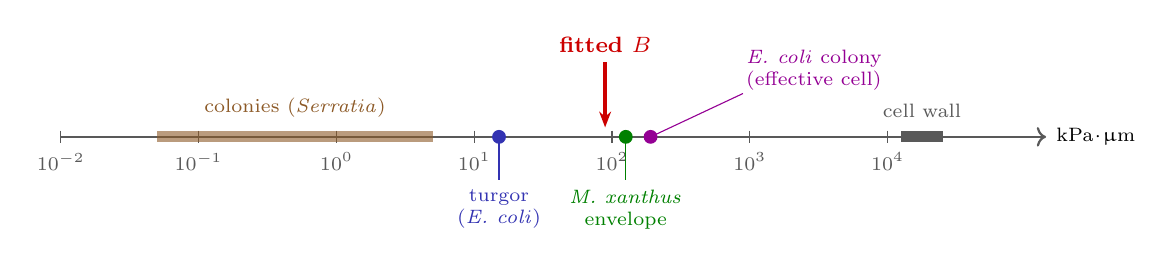
\begin{tikzpicture}[x=1.75cm,y=1cm,font=\scriptsize]
  % x = log10(value in kPa um) + 2
  \draw[->,thick,softgray] (0,0) -- (7.15,0) node[right,black] {$\kPa\tcdot\micron$};
  \foreach \e in {-2,...,4}{
    \draw[softgray] (\e+2,0.08) -- (\e+2,-0.08);
    \node[below,softgray] at (\e+2,-0.08) {$10^{\e}$};}
  % colonies of Serratia: 0.05-5
  \draw[line width=4pt,laneS,opacity=0.6] (0.70,0) -- (2.70,0);
  \node[above,text=laneS] at (1.7,0.12) {colonies (\textit{Serratia})};
  % E. coli turgor: 15
  \fill[bblue] (3.18,0) circle (2.5pt);
  \draw[bblue] (3.18,0) -- (3.18,-0.55) node[below,align=center] {turgor\\ (\textit{E.\ coli})};
  % M. xanthus envelope: 125
  \fill[darkgreen] (4.10,0) circle (2.5pt);
  \draw[darkgreen] (4.10,0) -- (4.10,-0.55) node[below,align=center] {\textit{M.\ xanthus}\\ envelope};
  % E. coli colony fit: 190
  \fill[purple] (4.28,0) circle (2.5pt);
  \draw[purple] (4.28,0) -- (4.95,0.55) node[above right,inner sep=1pt,align=left] {\textit{E.\ coli} colony\\ (effective cell)};
  % cell wall: 1.25e4-2.5e4
  \draw[line width=4pt,softgray] (6.10,0) -- (6.40,0);
  \node[above,text=softgray] at (6.25,0.12) {cell wall};
  % fitted B: 90
  \draw[darkred,very thick,-{Stealth[length=2mm]}] (3.95,0.95) -- (3.95,0.12);
  \node[above,text=darkred,font=\footnotesize\bfseries] at (3.95,0.95) {fitted $B$};
\end{tikzpicture}
\note{[1:15]
The last four parameters belong to the model and have no direct measurement. The rotational friction we estimate as for a rigid rod of 6 $\upmu$m. The relaxation rate of the nematic order must exceed 5 per minute for the free energy to be stable, and we take 10, so the order relaxes over about six seconds. The cutoff $\ell_\text{n}$ is the width of one cell, 0.5 $\upmu$m, the shortest length in the monolayer; the result depends on it, as we will see.

\clk The bulk modulus $B$ is the one parameter we fit, to the height of the measured peak. On this log scale are moduli of related systems, multiplied by the layer height: colonies of \textit{Serratia} on agar at the soft end, the turgor pressure of \textit{E.\ coli}, the envelope stiffness of \textit{M.\ xanthus} from indentation, the effective cell modulus that fits growing \textit{E.\ coli} colonies, and the cell wall at the stiff end. Our $B$ is stiffer than the colonies and of the order of the stiffness of single cells.}
\end{frame}


\begin{frame}[t,label=m-steady]{Steady state of a $+1/2$ defect}
\small\setlength{\abovedisplayskip}{3pt}\setlength{\belowdisplayskip}{3pt}
\begin{columns}[T,totalwidth=\textwidth]
\column{0.5\textwidth}
\onslide<+->
Noiseless, without the cross-coupling: static
\[0=\nabla\cdot\big[B\nabla\rho-\colA{\fa}\big],\qquad \Ha=0\]
Nematic field: Pad\'e profile
\[\Q=S(r)\,\hat\Q(\phi/2),\qquad S:\;0\to S_0\text{ over }\elld\]
\onslide<+->
Density: Poisson equation, reservoir $\rho=1$ at $R=20~\micron$
\[\boxed{\rho=1-\frac{\zeta}{B}\Big[S(r)-\frac rR\,S(R)\Big]\cos\phi}\]
\column{0.5\textwidth}
\centering
\onslide<2->
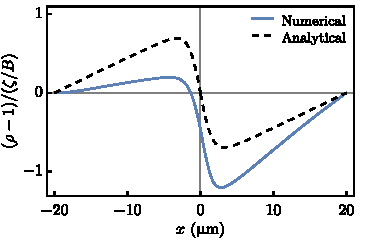
\includegraphics[width=\linewidth]{rho1d_Dirichlet}\\[-0.3ex]
{\scriptsize along the axis $y=0$, head at $x<0$;\; numerical: full comoving solution}
\end{columns}

\vspace{1ex}
\onslide<+->
\centering
\msg{mean density changes only by $\zeta/B\approx10^{-4}$ $\Rightarrow$ mean pressure $\sim\zeta\approx10~\Pa\tcdot\micron$, \;vs.\ $p_\text{crit}=35~\kPa\tcdot\micron$}
\hfill\tobackup{b-walls}{boundary}
\note{[1:15]
First the noiseless steady state of a $+1/2$ defect, with the head on the left. If we drop the cross-coupling, the problem is static. The nematic part, $\mathbf H^\text{a}=0$, is solved by the standard Pad\'e profile: the order rises from zero at the core to $S_0$ over the core size $\ell_\text{d}$.

\clk The density then obeys a Poisson equation, driven by the divergence of the active force. Its solution needs a boundary, and we take a reservoir, $\rho=1$ on a circle of 20 $\upmu$m, about the nematic correlation length. The solution is exact, and the plot compares it with the full numerics.

\clk The message is the scale on the $y$ axis: the density departs from one only by $\zeta/B$, about $10^{-4}$, so the mean pressure is of the order of $\zeta$, about 10 Pa$\cdot\upmu$m, three to four orders of magnitude below $p_\text{crit}$.}
\end{frame}


\begin{frame}[t,label=m-drift]{The defect moves}
\small\setlength{\abovedisplayskip}{3pt}\setlength{\belowdisplayskip}{3pt}
\begin{columns}[T,totalwidth=\textwidth]
\column{0.46\textwidth}
\centering
\begin{tikzpicture}[scale=0.8]
  \plusdefect
  \node[font=\scriptsize,softgray] at (-2.0,2.4) {head};
  \node[font=\scriptsize,softgray] at (2.0,2.4) {tail};
  \draw[darkred,line width=2.5pt,-{Stealth[length=3mm]}] (0.15,0.3) -- (-1.3,0.3)
     node[above,font=\scriptsize,align=center,fill=white,inner sep=1pt] {active force};
  \only<2->{\draw[bblue,line width=2.5pt,-{Stealth[length=3mm]}] (-0.15,-0.3) -- (1.3,-0.3)
     node[below,font=\scriptsize,align=center,fill=white,inner sep=1pt] {model: $+0.24~\micron/\minute$};}
  \only<3->{\draw[darkgreen,line width=2.5pt,dashed,-{Stealth[length=3mm]}] (-0.3,-1.25) -- (-1.75,-1.25)
     node[below,font=\scriptsize,fill=white,inner sep=1pt] {experiments};}
\end{tikzpicture}
\column{0.54\textwidth}
\onslide<+->
Active force along the axis, toward the head:
\[\colA{f^\mathrm a_x=-\zeta\,\big(S'+S/r\big)},\qquad \colA{f^\mathrm a_y=0}\]
cells pile up at the head until $B\nabla\rho\simeq\colA{\fa}$

\vspace{1ex}
\onslide<+->
Cross-coupling in the $\Q$ equation:
\[\frac{B}{\xi_0}\nabla\cdot(\Q\nabla\rho)\;:\;\text{carries }\Q\text{ with }-\frac{B\nabla\rho}{\xi_0}\;\to\;\text{tail}\]
comoving solution: $u_x=+0.24~\micron/\minute$, toward the \textbf{tail}

\vspace{1ex}
\onslide<+->
{\color{darkgreen} experiments: $+1/2$ defects move toward their \textbf{head}}
\end{columns}
\note{[1:15]
Now restore the cross-coupling. The active force at a $+1/2$ defect points along the axis, toward the head, and it is largest at the core. It pushes the cells toward the head, until the pressure gradient balances it.

\clk Within our closure, however, the nematic order is carried by the pressure-driven flow, whose velocity $-B\nabla\rho/\xi_0$ points against the active force. So the defect itself moves toward its tail, at 0.24 $\upmu$m/min in our box.

\clk In the experiments, $+1/2$ defects move the other way, toward their head. The difference comes from the closure, as I show in two slides.}
\end{frame}


\begin{frame}[t]{The moving defect stays close to the Pad\'e profile}
\begin{columns}[T,totalwidth=\textwidth]
\column{0.42\textwidth}
\centering
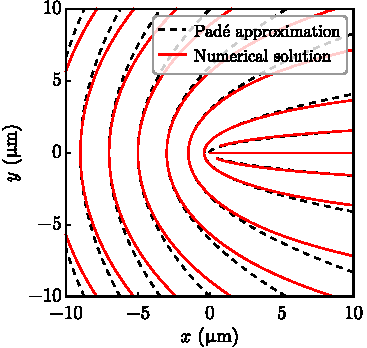
\includegraphics[width=\linewidth]{nematicaxis}\\
{\scriptsize director lines}
\column{0.56\textwidth}
\centering
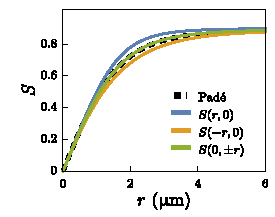
\includegraphics[width=0.49\linewidth]{strength}\hfill
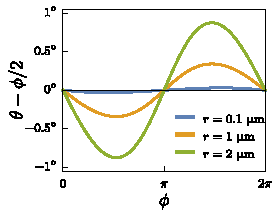
\includegraphics[width=0.49\linewidth]{defectangle}\\
{\scriptsize order $S$ along and across the axis \hfill director angle vs.\ Pad\'e}

\vspace{2ex}
\raggedright\small
\begin{itemize}\setlength{\itemsep}{1ex}
\item near the core: director within $1^\circ$, $S$ within $6\%$ of $S_0$
\item farther out: director lines separate
\item variance evaluated on both profiles
\end{itemize}
\end{columns}
\note{[0:40]
The motion also deforms the defect. Near the core the deformation is small: the director stays within a degree of the static profile, and the order changes by at most 6\% of $S_0$. Farther out, the director lines of the moving defect separate from the Pad\'e profile. For the fluctuations we use both profiles.}
\end{frame}


\begin{frame}[t,label=m-Y]{What the closure drops: alignment carried along the rods}
\small\setlength{\abovedisplayskip}{3pt}\setlength{\belowdisplayskip}{3pt}
\begin{columns}[T,totalwidth=\textwidth]
\column{0.62\textwidth}
\onslide<+->
Rods diffuse along their own axis ($D_\parallel=v_0^2/2\frev$) and carry their alignment. In the exact $\Q$ equation:
\[\colA{\frac{\zeta}{\xi_0}}\Big(\lab{\nabla^2Q_\ab}{isotropic: in $K'$}+\lab{\partial_\mu\partial_\nu\langle\hat Q_\ab\hat Q_\mn\rangle_\varrho}{along the rod axis}\Big)\]
\onslide<+->
lowest order, $\langle\hat\Q\hat\Q\rangle_\varrho\simeq\rho\J$: \;$\frac{\zeta}{\xi_0}\big(\partial_\alpha\partial_\beta-\tfrac12\delta_\ab\nabla^2\big)\rho$\\
{\footnotesize\color{softgray} only $\nabla\nabla\rho$, smaller than the cross-coupling by $\zeta/B$ $\Rightarrow$ dropped}\\[0.8ex]
\onslide<+->
exact, $\langle\hat\Q\hat\Q\rangle_\varrho=\rho\J+\frac{g_2}{2\rho}\U(\Q)$, adds
\[\boxed{\Y_\ab=\frac{\zeta}{\xi_0}\,\partial_\mu\partial_\nu\Big[\frac{g_2}{2\rho}\,U_{\ab\mu\nu}(\Q)\Big]}\]
{\footnotesize $\U=2\big[\Q\Q-\tfrac12(\Q\!:\!\Q)\J\big]$, fourth harmonic: $g_2S^2=0.66$ at $S=0.9$;\; no $\nabla\rho$, so $B$ does not suppress it: near the core as large as the cross-coupling}
\column{0.38\textwidth}
\centering
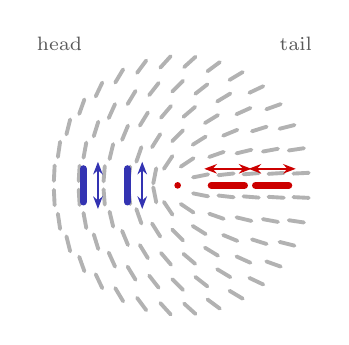
\begin{tikzpicture}[scale=0.75]
  \plusdefect
  \node[font=\scriptsize,softgray] at (-2.0,2.4) {head};
  \node[font=\scriptsize,softgray] at (2.0,2.4) {tail};
  \onslide<1->{
  % tail: rods along the axis, diffuse along x, into the core
  \foreach \xx in {0.85,1.6}{
    \draw[rod=darkred] (\xx-0.28,0) -- (\xx+0.28,0);
    \draw[darkred,thick,{Stealth[length=1.6mm]}-{Stealth[length=1.6mm]}] (\xx-0.4,0.28) -- (\xx+0.4,0.28);}
  % head: rods across the axis, diffuse along y
  \foreach \xx in {-0.85,-1.6}{
    \draw[rod=bblue] (\xx,-0.28) -- (\xx,0.28);
    \draw[bblue,thick,{Stealth[length=1.6mm]}-{Stealth[length=1.6mm]}] (\xx+0.25,-0.4) -- (\xx+0.25,0.4);}
  }
\end{tikzpicture}\\[0.5ex]
{\scriptsize\raggedright
\colA{tail}: rods along the axis carry their alignment into the core\\
\colI{head}: rods across the axis carry it sideways\\}
\end{columns}
\note{[1:45]
What did the closure drop? With reversals, each rod diffuses along its own axis, and it carries its alignment with it. At the tail of the defect the rods lie along the axis and carry their alignment into the core; at the head they lie across the axis and carry it sideways.

In the $\Q$ equation this transport is the self-propulsion term. Its first part is isotropic and only renormalizes the elastic constant. The second part depends on the angular distribution of the rods, through $\la\hat\Q\hat\Q\ra$.

\clk With the lowest-order closure this part involves only density gradients, which are small, of order $\zeta/B$, so it drops out.

\clk With the exact moments of the von Mises distribution, an extra term survives: $\mathbf Y$, which involves the fourth angular harmonic of the distribution. It contains no density gradient, so the large $B$ does not suppress it, and at $S=0.9$ its amplitude $g_2S^2$ is 0.66. Near the core it is as large as the cross-coupling that moves the defect. So the lowest-order closure drops a term as large as the one that sets the drift.}
\end{frame}


\begin{frame}[t,label=m-reverse]{Adding $\Y$ reverses the drift}
\small\setlength{\abovedisplayskip}{3pt}\setlength{\belowdisplayskip}{3pt}
\onslide<+->
\[\partial_t\Q=\frac4{\xir}\Ha+\lab{\frac{B}{\xi_0}\nabla\cdot(\Q\nabla\rho)}{cross-coupling: $\to$ tail}+\lab{\mathhlbox{liteyellow}{w\,\Y}}{$\to$ head},
\qquad w:\;0\;\text{(our closure)}\to1\;\text{(exact moments)}\]
\onslide<+->
{\scriptsize on the defect, $\Psi=Q_{xx}+\ii Q_{xy}$:\;
$Y_{xx}+\ii Y_{xy}=\frac{\zeta}{2\xi_0}\,\bar\partial^{\,2}\big(g_2\Psi^2/\rho\big)$,\;
at the core $\approx2\times$ the cross-coupling, opposite sign}

\onslide<+->
\begin{columns}[T,totalwidth=\textwidth]
\column{0.52\textwidth}
\centering
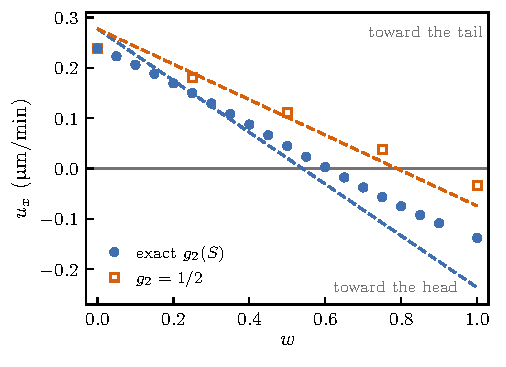
\includegraphics[width=0.72\linewidth]{drift_closure}
\column{0.46\textwidth}
\centering
\onslide<+->
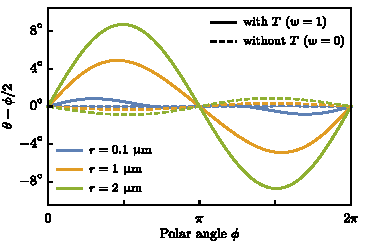
\includegraphics[width=0.78\linewidth]{drift_deformation}\\
{\scriptsize director angle near the core; $T$ in the legend $=\Y$}
\end{columns}
\onslide<3->
\centering
{\small at $w=1$: $u_x=-0.14~\micron/\minute$, toward the \textbf{head}, as in experiments}\hfill\tobackup{b-estimate}{estimate}
\note{[1:15]
We add $w\mathbf Y$ to the $\Q$ equation and follow the steady state as $w$ goes from 0, our closure, to 1, the exact moments in this one term. Everything else stays the same.

\clk On the defect, $\mathbf Y$ is a source of $Q_{xx}$ at the core, about twice the cross-coupling and of opposite sign.

\clk The drift velocity decreases with $w$ and changes sign near $w=0.6$. At $w=1$ the defect moves toward its head at 0.14 $\upmu$m/min, as in the experiments. The dashed lines are a first-order estimate, which overshoots but gets the trend.

\clk With $\mathbf Y$ the director near the core rotates by several degrees, on the sides of the defect; $T$ in the legend is this $\mathbf Y$. We did not recompute the fluctuations on this state, so what follows uses our closure.}
\end{frame}


\begin{frame}[t,label=m-pedestal]{Density fluctuations: the pedestal}
\small\setlength{\abovedisplayskip}{3pt}\setlength{\belowdisplayskip}{3pt}
\onslide<+->
Linearize about the steady state; freeze the nematic fluctuations, $\delta\Q=0$\\
{\footnotesize\color{softgray} at the cell scale $\delta\Q$ relaxes $\sim10^4$ times slower than $\delta\rho$: the density follows it quasi-statically}
\[\partial_t\delta\rho=\gamma_0\nabla^2\delta\rho-\nabla\cdot\colA{\bEta_\rho},\quad\gamma_0=\frac{B}{\xi_0}
\qquad\onslide<2->{\Rightarrow\qquad
\delta\tilde\rho(\k,\omega)=-\frac{\ii\,\k\cdot\colA{\tilde\bEta_\rho}}{\ii\omega+\gamma_0k^2}}\]
\onslide<+->
noise power $\propto k^2$, relaxation $\propto k^2$ $\Rightarrow$ flat spectrum: the variance at a point diverges\\[0.5ex]
\onslide<+->
cutoff at the width of one cell, $\elln=0.5~\micron$ \;{\footnotesize (Gaussian filter $\ee^{-k^2\elln^2/4}$)}
\onslide<+->
\[\boxed{\sigma_\rho^2\big|_\text{pedestal}=\frac{\zeta}{2\pi B\rho_0\elln^2}},\qquad
\text{correlation time } \tau_c=\frac{\elln^2}{2\gamma_0}\approx0.4~\text{ms}\]
\onslide<+->
\centering
\msg{$\sigma_\rho\propto B^{-1/2}$\; vs.\ mean profile $\propto B^{-1}$:\quad $\sigma_\rho\approx2\%$ vs.\ $\zeta/B\approx10^{-4}$ \;$\Rightarrow$ fluctuations swamp the mean}\\[1ex]
{\footnotesize uniform order leaves the one-point variance unchanged; only how the order \emph{varies} around a point modulates it}
\hfill\tobackup{b-cutoff}{cutoff}
\note{[1:30]
Now the fluctuations. We linearize around the steady state and, for the analytic result, freeze the nematic fluctuations. At the scale of a cell the order relaxes nearly four orders of magnitude more slowly than the density, so the density follows it quasi-statically.

\clk In Fourier space, the noise is a flux, so its power carries $k^2$, and the pressure relaxes the density at the rate $\gamma_0k^2$. The two cancel, the spectrum is flat, and the variance at a point diverges: a continuum fluctuates at every scale.

\clk But the monolayer has no length shorter than the width of a cell, so we cut off there, at $\ell_\text{n}=0.5$ $\upmu$m.

\clk Then the variance far from defects is a constant pedestal, $\zeta/(2\pi B\rho_0\ell_\text{n}^2)$. A fluctuation of size $\ell_\text{n}$ lives for $\tau_c\approx0.4$ ms.

\clk Note the scaling: the standard deviation goes as $B^{-1/2}$, whereas the mean profile goes as $B^{-1}$. At our $B$ the density fluctuates by about 2\%, against $10^{-4}$ for the mean. And uniform order leaves the variance at a point unchanged, so only the variation of the order around a point, as at a defect, can modulate it.}
\end{frame}


\begin{frame}[t,label=m-variance]{Density variance around a $+1/2$ defect}
\small\setlength{\abovedisplayskip}{3pt}\setlength{\belowdisplayskip}{3pt}
\begin{columns}[T,totalwidth=\textwidth]
\column{0.5\textwidth}
\onslide<+->
noise $\propto\big[\Q_\ss+\I\big]$: stronger along the rods
\[\frac{\sigma_\rho^2(\r)}{\sigma_\rho^2|_\text{pedestal}}=1+\frac{\elln^2}{4}\big(\kappa\star\partial_i\partial_jQ^\ss_{ij}\big)(\r)\]
\onslide<+->
integrate by parts:
\[\boxed{\frac{\sigma_\rho^2(\r)}{\sigma_\rho^2|_\text{pedestal}}=1+\big\langle S\cos2(\theta_\text{nb}-\theta_{\bs d})\big\rangle_\Omega}\]
{\footnotesize average over neighbours $\r+\bs d$, with weight}
\[\Omega(d)=\frac{\elln^2}{2\pi d^4}\Big[2-\ee^{-X}\big(X^2+2X+2\big)\Big],\quad X=\frac{2d^2}{\elln^2}\]
{\footnotesize $\int\!\d^2\bs d\,\Omega=1$,\; $\Omega(0)=0$}
\column{0.5\textwidth}
\onslide<+->
\centering
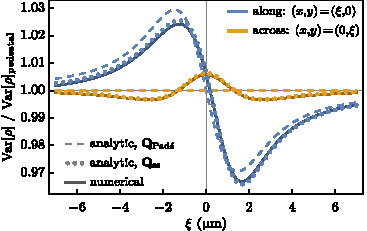
\includegraphics[width=\linewidth]{varrho}\\[0.5ex]
{\footnotesize head ($x<0$): $+2.4\%$ at $1.25~\micron$\\ tail: $-3.3\%$ at $1.7~\micron$}\\[0.5ex]
{\scriptsize dashed: formula on Pad\'e;\; dots: formula on $\Q_\ss$;\\ solid: numerics with $\delta\Q\neq0$}
\hfill\tobackup{b-solver}{solver}
\end{columns}
\note{[1:20]
Near the defect the noise is anisotropic, stronger along the rods. The anisotropic part of the variance is the double divergence of the nematic field, smoothed over a few $\ell_\text{n}$.

\clk Integrating by parts turns it into one simple expression: the variance relative to the pedestal is one plus an average over the neighbours of the point of $S\cos2(\theta_\text{nb}-\theta_d)$. The weight $\Omega$ depends only on the distance, vanishes at the point itself, and reaches about 2 $\upmu$m.

\clk Along the axis, the variance is raised by 2.4\% about 1.25 $\upmu$m from the core on the head side, and lowered by 3.3\% on the tail side. The dashed curve is this formula on the Pad\'e profile, the dots the formula on the moving defect, and the solid line the full numerics with nematic fluctuations. The formula captures the numerics; most of the small remaining difference comes from the grid.}
\end{frame}


\begin{frame}[t]{Density variance: the map}
\centering
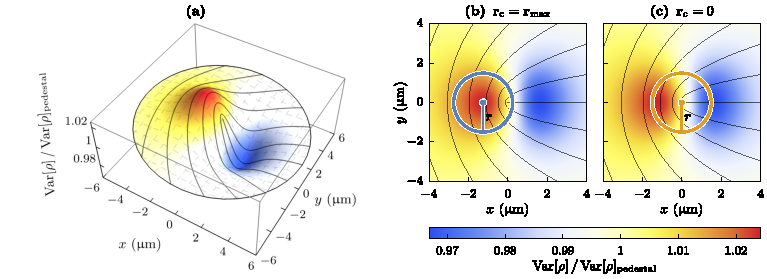
\includegraphics[width=\linewidth]{variance_map}\\[1ex]
{\small maximum off the core, at the head;\; minimum at the tail\\
(b, c): circles over which the layering probability is averaged}
\note{[0:30]
Here is the full two-dimensional map from the numerics. The maximum is off the core, at the head; the minimum is at the tail. Panels b and c show the circles over which we will average the layering probability, centred on the maximum or on the core.}
\end{frame}


\begin{frame}[t]{Why: a cell runs along its own axis}
\centering
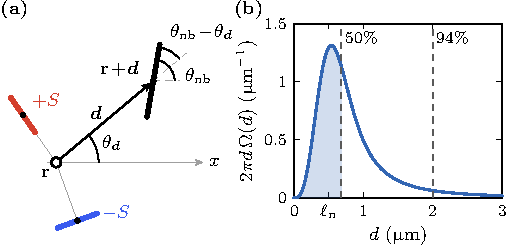
\includegraphics[width=0.82\linewidth]{neighbor_diagram_v3}

\vspace{1ex}
\small\raggedright
\begin{itemize}\setlength{\itemsep}{0.5ex}
\item<1-> a cell moves density into and out of the points \textbf{ahead} and \textbf{behind}, not beside it
\item<1-> neighbour rod pointing at $\r$: \colA{$+S$};\quad across the line to $\r$: \colI{$-S$}
\item<2-> half the weight within $0.68~\micron$, $94\%$ within $2~\micron$;\; uniform nematic: they balance
\end{itemize}
\note{[1:00]
Why this pattern? A cell runs back and forth along its own axis, so it moves density into and out of the points ahead of it and behind it, not those beside it. A neighbour whose rod points at $\r$ therefore adds to the variance at $\r$, with $+S$, and one whose rod lies across the line to $\r$ subtracts, with $-S$.

\clk The weight of a neighbour depends only on its distance: half of the weight lies within 0.68 $\upmu$m, and 94\% within 2 $\upmu$m. In a uniform nematic the two kinds of neighbours balance exactly.}
\end{frame}


\begin{frame}[t,label=m-aimed]{Neighbours that raise and lower the variance}
\centering
\begin{tikzpicture}
  \node[anchor=south west,inner sep=0pt] (img) at (0,0)
    {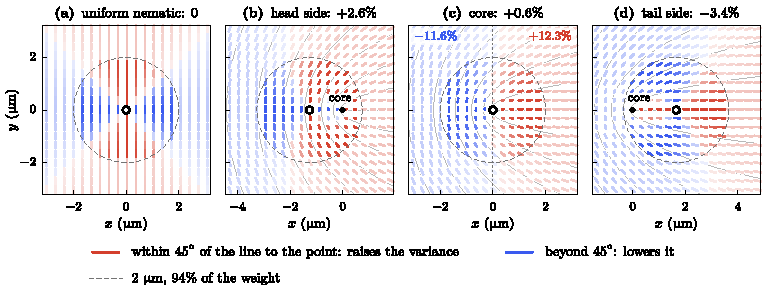
\includegraphics[width=\linewidth]{aimed_rods_qss}};
  % white covers hide the panels not yet discussed; the legend (bottom 19%) stays
  \begin{scope}[shift={(img.south west)},x={($(img.south east)-(img.south west)$)},y={($(img.north west)-(img.south west)$)}]
    \only<1>{\fill[cover] (0.285,0.19) rectangle (1.001,1.001);}
    \only<2>{\fill[cover] (0.524,0.19) rectangle (1.001,1.001);}
    \only<3>{\fill[cover] (0.764,0.19) rectangle (1.001,1.001);}
  \end{scope}
\end{tikzpicture}

\vspace{1.5ex}
\small
\only<1>{\textbf{(a)} uniform nematic: red and blue neighbours balance}%
\only<2>{\textbf{(b)} head side: between the point and the core the lines bend around the core,\\ so the rods turn \emph{toward} the point; beyond it they bend back, but less}%
\only<3>{\textbf{(c)} core: head side $-11.6\%$, tail side $+12.3\%$;\\ they cancel on the Pad\'e profile, the tail wins in the moving defect}%
\only<4>{\textbf{(d)} tail side: the rods between the point and the core turn \emph{away} from the point}\\[1ex]
{\scriptsize panel titles: the formula on the moving defect $\Q_\ss$ (dots of the previous plot)}
\note{[1:30]
This is the picture around the defect: each panel shows the rods around one point, coloured by the sign with which they count; red raises the variance, blue lowers it.

(a) In a uniform nematic, red and blue balance.

\clk (b) At the maximum on the head side, the director lines between the point and the core bend around the core, so the rods above and below the axis turn toward the point and raise the variance. Beyond the point the lines bend the other way, but less, so those rods only partly offset them.

\clk (c) At the core, the head and the tail side nearly cancel. On the static Pad\'e profile they cancel exactly; in the moving defect the tail side, where the order is stronger, wins slightly.

\clk (d) On the tail side, the rods between the point and the core turn away from the point and lower the variance. So the head--tail asymmetry comes from the geometry of the director field, and its fine details from the motion of the defect.}
\end{frame}


\begin{frame}[t,label=m-minus]{The $-1/2$ defect: weaker, and farther out}
\small
\begin{columns}[T,totalwidth=\textwidth]
\column{0.58\textwidth}
\centering
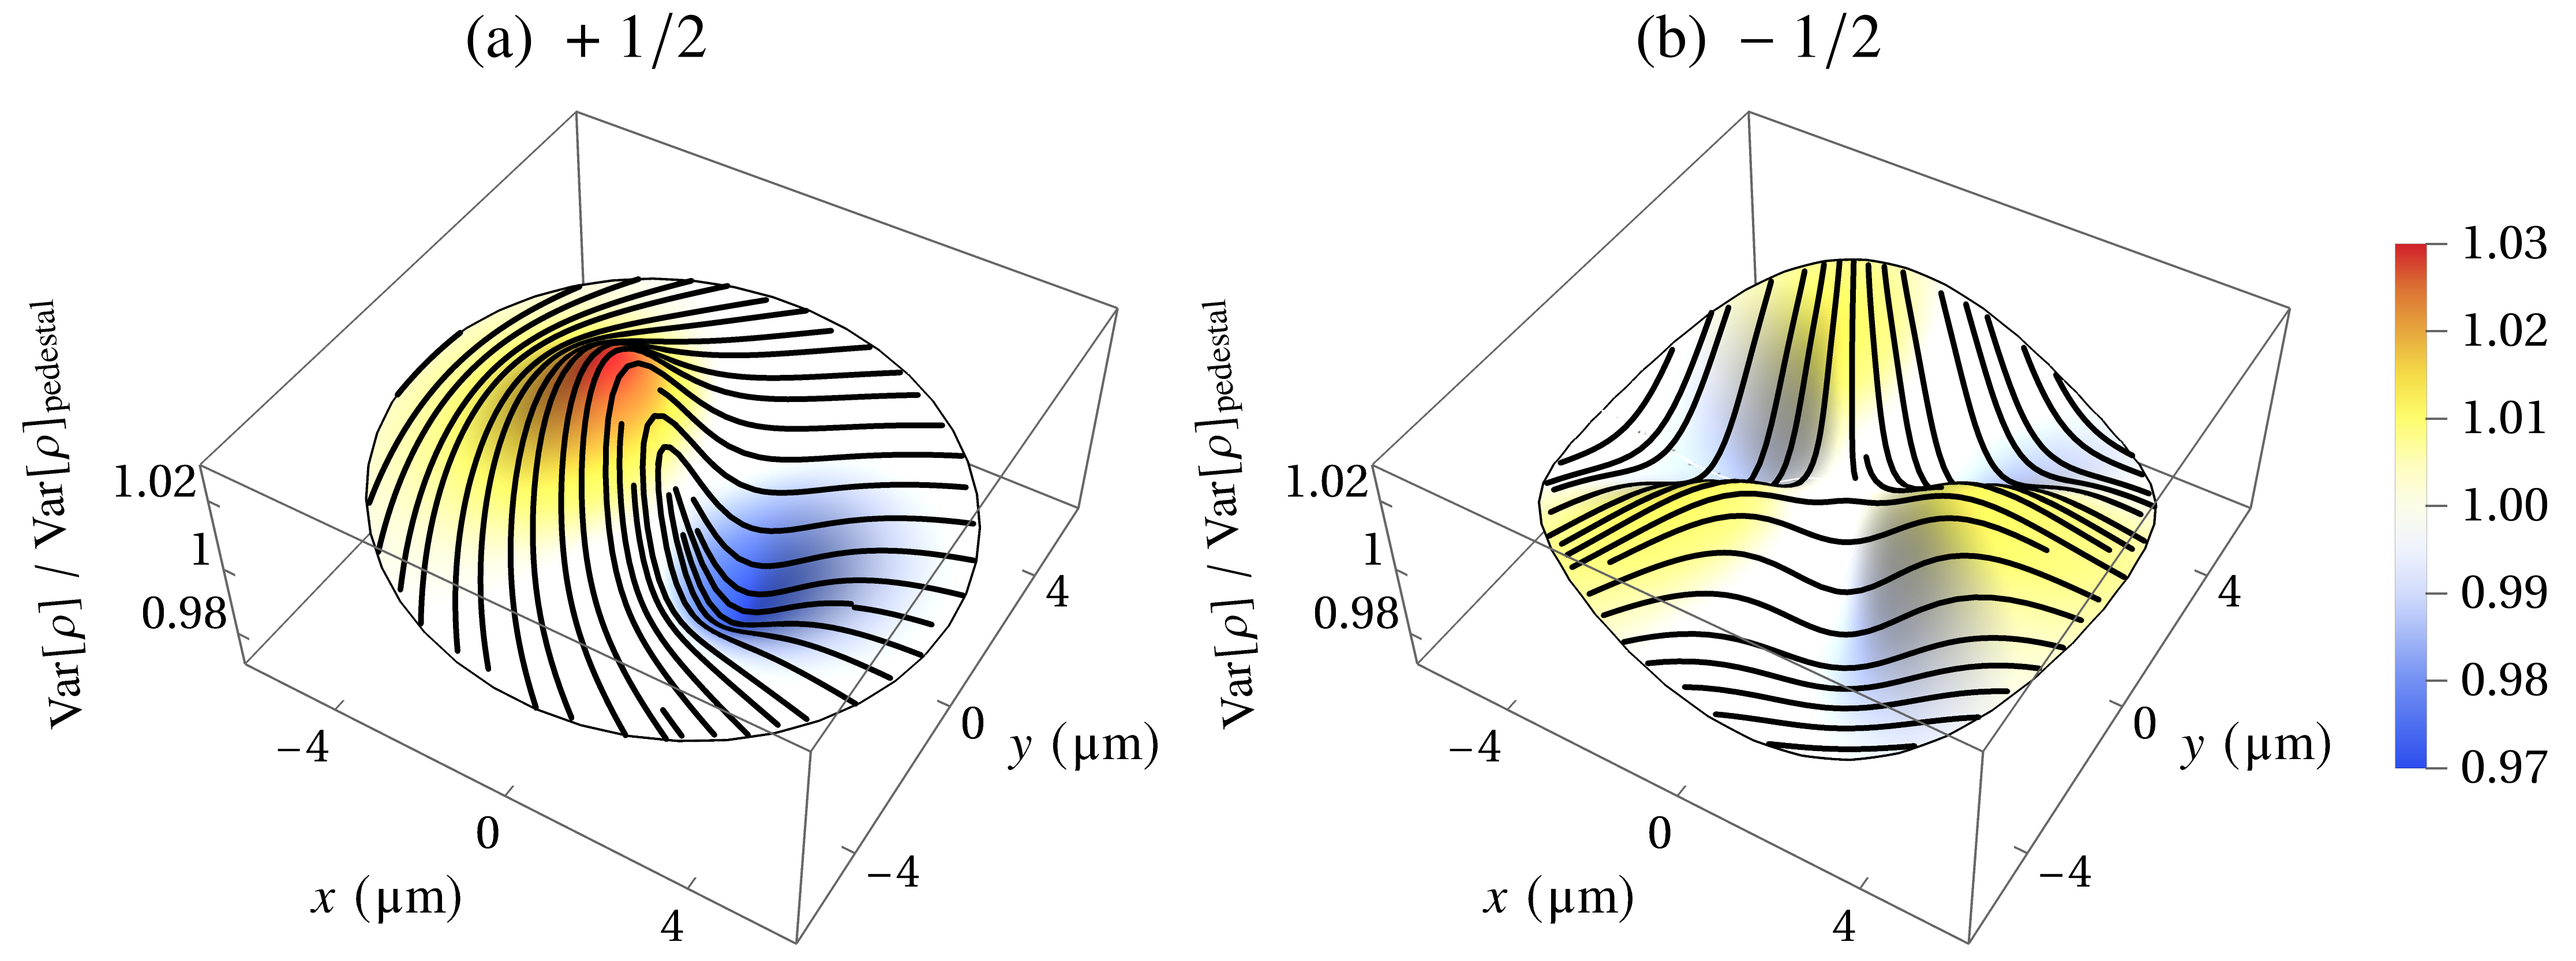
\includegraphics[width=\linewidth]{varrho3D_pm}\\
{\scriptsize analytic, $\delta\Q=0$, Pad\'e profiles, same parameters}

\vspace{1ex}
\raggedright
\begin{itemize}\setlength{\itemsep}{0.5ex}
\item threefold: three raised lobes (director radial), three lowered (director around the core)
\item peak $1.35\%$ at $3.3~\micron$, vs.\ $2.94\%$ at $1.5~\micron$ for $+1/2$
\item near the core $\propto r^3$, vs.\ $\propto r$ for $+1/2$
\end{itemize}
\column{0.4\textwidth}
\onslide<2->
\centering
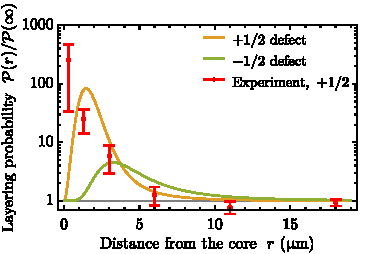
\includegraphics[width=\linewidth]{layering_pm}\\
{\scriptsize averaged over circles about the core}

\vspace{1ex}
\raggedright
model: more layers near $-1/2$ too, but less, and farther out

\vspace{1ex}
{\color{darkred} experiments: mainly \textbf{holes} at $-1/2$ ($\approx80\times$)}\\
$\Rightarrow$ needs additional modelling
\end{columns}
\note{[1:15]
The same formula applies to a $-1/2$ defect. Its director has threefold symmetry, so the variance has three raised lobes, where the director points radially, and three lowered lobes between them. The peak is 1.35\%, less than half the $+1/2$ value, and more than twice as far from the core, at 3.3 $\upmu$m: close to the core, the neighbours of a point reach into the lowered lobes on both sides, which nearly cancel the raised one. Near the core the modulation grows only as $r^3$, against $r$ for the $+1/2$ defect.

\clk So the model raises the layering probability near $-1/2$ defects too, but less and farther out, as the plot shows. In the experiments, however, mainly holes open at $-1/2$ defects, about 80 times more often than far away. Explaining the holes needs additional modelling.}
\end{frame}


\begin{frame}[t,label=m-layering]{Layer formation}
\small\setlength{\abovedisplayskip}{3pt}\setlength{\belowdisplayskip}{3pt}
\begin{columns}[T,totalwidth=\textwidth]
\column{0.53\textwidth}
\onslide<+->
$\delta p=B\,\delta\rho$ is Gaussian, with
\[\sigma_p^2(\r)=B^2\sigma_\rho^2(\r),\qquad \sigma_{p,\infty}=1.7~\kPa\tcdot\micron\]
\onslide<+->
Gaussian tail, $z=p_\text{crit}/\sigma_p$:\quad $\calP(\r)\propto\dfrac{\ee^{-z^2/2}}{\sqrt{2\pi}\,z}$,\quad $z_\infty=20.8$
\[\frac{\calP(\r)}{\calP(\infty)}\simeq\exp\Big[\frac{z_\infty^2}{2}\Big(1-\frac{\sigma_{p,\infty}^2}{\sigma_p^2(\r)}\Big)\Big]\]
{\footnotesize the relative change of the variance is multiplied by $z_\infty^2/2\approx200$}\\[1ex]
\onslide<+->
peak, $\nu_0=2.4\%$:
\[\frac{\calP(\r_\text{max})}{\calP(\infty)}=\exp\Big[\frac{z_\infty^2}{2}\,\frac{\nu_0}{1+\nu_0}\Big]\approx\boxed{1.7\times10^2}\]
\centering{\color{darkred} measured: $\approx2\times10^2$}
\column{0.46\textwidth}
\onslide<+->
\centering
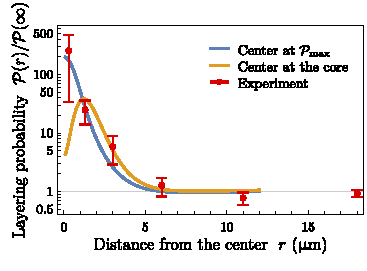
\includegraphics[width=0.9\linewidth]{layering_profile}\\
{\scriptsize averaged over circles of radius $r$;\\ data: Fig.~3f of Copenhagen et al.\ 2021}

\vspace{0.5ex}
\raggedright\footnotesize
\begin{itemize}\setlength{\itemsep}{0.2ex}
\item one fitted parameter, $B$: it sets only the height
\item shape: from the defect profile and $\elln$
\item absolute rate: out of reach, $\propto\ee^{-z_\infty^2/2}$
\end{itemize}
\end{columns}
\note{[1:30]
Finally, layer formation. A density fluctuation changes the pressure by $B\,\delta\rho$, so the pressure is Gaussian with $B^2$ times the density variance. Far from defects $\sigma_p$ is 1.7 kPa$\cdot\upmu$m.

\clk The critical pressure lies 20.8 standard deviations out, so the layering probability is the far tail of the Gaussian. In the ratio to the far field only the relative change of the variance enters, multiplied by $z_\infty^2/2$, about 200.

\clk So a modulation of 2.4\% becomes an enhancement of $1.7\times10^2$ at the maximum, close to the measured $2\times10^2$.

\clk On the right, the probability averaged over circles, centred on the maximum, in blue, or on the core, in orange, against the data of Copenhagen et al.\ We show both, because we do not know which centre the measurement corresponds to. The only fitted parameter is $B$, and it sets only the height; the shape follows from the defect profile and the cutoff. The absolute rate is out of reach: it depends exponentially on $z_\infty^2$, so a small change of $\sigma_p$ or $p_\text{crit}$ changes it by orders of magnitude.}
\end{frame}


% ===========================================================================
% Closing
% ===========================================================================
\begin{frame}[t]{Summary}
\onslide<+->
\centering
{\color{darkgreen} Polarity fluctuations $\;\longrightarrow\;$ Pressure fluctuations $\;\longrightarrow\;$ \textbf{Nucleation theory}}

\vspace{1ex}
\raggedright\small
\begin{itemize}\setlength\itemsep{0.6ex}
\item mean pressure at a defect $\sim10^{-3}$--$10^{-4}\,p_\text{crit}$: layers need rare \textbf{fluctuations}
\item reversing rods $\to$ Dean's equation $\to$ fluctuating active nematic:\\ the same $\zeta=\xi_0v_0^2/4\frev$ sets the active stress and the noise
\item density variance $+2$--$3\%$ off the core, at the \textbf{head} of a $+1/2$ defect
\item Gaussian tail: layering $\times1.7\times10^2$, one fitted parameter $B$
\end{itemize}

\vspace{1.5ex}
\onslide<+->
{\color{bblue} Open questions}
\begin{itemize}\setlength\itemsep{0.4ex}
\item closure at strong order: sets the drift direction and the head--tail asymmetry
\item white-noise reversals: minutes, vs.\ density relaxation within $\sim$1~ms at the cell scale
\item Gaussian statistics at the scale of one cell;\; idealized nucleus
\end{itemize}
\note{[1:20]
To summarize. The mean pressure at a defect is three to four orders of magnitude below the critical pressure, so we proposed that layers form during rare pressure fluctuations. We derived these fluctuations from reversing rods with Dean's equation, and the same coefficient $\zeta$ sets the active stress and the noise. The density variance is raised by a few percent off the core, at the head of a $+1/2$ defect, and lowered at its tail. The Gaussian tail amplifies this to two orders of magnitude in the layering probability, with one fitted parameter.

\clk The open questions are the simplifications. The closure at strong order sets the direction of the drift and the head--tail asymmetry. The white-noise limit is far from the real reversals: cells reverse every few minutes, whereas at the cell scale the density relaxes within a millisecond. And we use Gaussian statistics at the scale of one cell, with an idealized nucleus.}
\end{frame}


\begin{frame}[t,label=m-tests]{What experiments could test}
\small
\begin{columns}[T,totalwidth=\textwidth]
\column{0.5\textwidth}
\onslide<+->
\textbf{1.\ Where layers start}\\
{\footnotesize model: maximum off the core, at the \textbf{head};\\ no quantitative angular profile yet}\\[0.5ex]
\includegraphics[height=2.9cm,page=2,trim={104 0 246 0},clip]{handmade/main}

\vspace{2ex}
\onslide<3->
\textbf{3.\ Traction}\hfill\tobackup{b-force}{force}\\
{\footnotesize our active-force fluctuations exceed the mean everywhere along the axis; a quantitative test needs the traction variance at the measured resolution}
\column{0.5\textwidth}
\onslide<2->
\textbf{2.\ Reversal rate}\\
{\footnotesize the same $\zeta$ sets the noise: at fixed defect shape}
\[\ln\frac{\calP(\r_\text{max})}{\calP(\infty)}\;\propto\;\frac{\frev}{v_0^2}\]
{\footnotesize slower reversals: more layers everywhere, less concentrated at defects;\; \textit{frzE} (reverses every $\sim$2~h) forms more multilayers [Han 2025]; around defects: not measured}

\vspace{2ex}
\onslide<4->
\textbf{4.\ Density variance}\\
{\footnotesize most direct, but a few \% at the cell scale needs an average over many defects; its size depends on the resolution $\elln$}
\end{columns}
\note{[1:30]
What could you measure? First, where around the defect layers start. The model puts the maximum off the core, at the head, as in this example, and the authors of the Copenhagen and Han papers told us that, in unpublished observations, layering starts more often at the head. But there is no quantitative angular profile yet.

\clk Second, the reversal rate. The same $\zeta$ sets the noise, so at fixed defect shape the logarithm of the enhancement goes as $f_\text{rev}/v_0^2$. Slower reversals should give more layers everywhere, but less concentrated at defects. The \textit{frzE} mutant, which reverses about every two hours, does form more multilayers, but layering around defects at several reversal rates would test the second half.

\clk Third, the traction. The fluctuations of our active force exceed its mean everywhere along the defect axis, as in the measured traction, but the traction also contains the pressure gradient, so a quantitative comparison needs the traction variance at the resolution of the measurement, which we have not computed.

\clk Fourth, the density variance itself. It is the most direct test, but a modulation of a few percent at the cell scale needs an average over many defects.}
\end{frame}


\begin{frame}
\centering
{\LARGE\color{bblue} Thank you}

\vspace{4ex}
{\small polarity fluctuations $\;\to\;$ pressure fluctuations $\;\to\;$ layers at the head of $+1/2$ defects}
\note{[0:05]
Thank you.}
\end{frame}


% ===========================================================================
% Backup
% ===========================================================================
\appendix

\begin{frame}[t,label=b-solver]{Backup: Lyapunov solver with $\delta\Q\neq0$}
\small\setlength{\abovedisplayskip}{3pt}\setlength{\belowdisplayskip}{3pt}
linearized equations: Ornstein--Uhlenbeck field theory for $\psi=(\delta\rho,\delta Q_1,\delta Q_2)$
\[\partial_t\psi=\A\psi+\bxi\quad\Rightarrow\quad \A\,\mathbf C+\mathbf C\,\A^\T+\mathbf N=0\qquad\text{(equal-time covariance $\mathbf C$)}\]
\begin{columns}[T,totalwidth=\textwidth]
\column{0.62\textwidth}
\footnotesize
\begin{itemize}\setlength{\itemsep}{0.6ex}
\item grid $200\times200$ on $[-20,20]^2~\micron^2$, $\Delta x=0.2~\micron$; dense $\mathbf C$: 115~GB
\item noise from the exact von Mises moments: a Gram matrix, so positive semidefinite
\item staggered grid: noise and drift share one difference operator $\Rightarrow$ flat spectrum on the grid
\item noise correlated over $\ell_\text{eff}$, $2\%$ above $\elln$, so that the pedestal is exact (right)
\item reservoir walls: $\delta\rho=\delta\Q=0$, noise flux open
\end{itemize}
\column{0.36\textwidth}
\centering
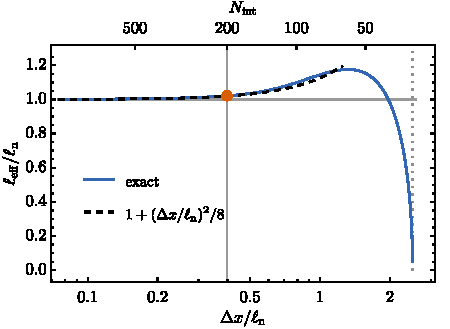
\includegraphics[width=\linewidth]{cutoff_calibration}
\end{columns}
\backto{m-variance}
\note{Backup. The linearized equations are an Ornstein--Uhlenbeck field theory, whose equal-time covariance solves a Lyapunov equation. The noise covariance needs the exact moments, otherwise it has a negative eigenvalue; the noise and the drift must use the same difference operator, otherwise the flat spectrum is lost at the grid scale; and the correlation length of the noise is calibrated so that the grid reproduces the continuum pedestal.}
\end{frame}


\begin{frame}[t,label=b-walls]{Backup: boundary condition of the steady state}
\small\setlength{\abovedisplayskip}{3pt}\setlength{\belowdisplayskip}{3pt}
\begin{columns}[T,totalwidth=\textwidth]
\column{0.5\textwidth}
closed forms on a disk of radius $R$:\\[1ex]
reservoir, $\rho=1$:
\[\rho=1-\frac{\zeta}{B}\Big[S(r)-\frac rR\,S(R)\Big]\cos\phi\]
no flux, $\nh\cdot(B\nabla\rho-\fa)=0$:
\[\rho=1-\frac{\zeta}{B}\Big[S(r)+\frac rR\,S(R)\Big]\cos\phi\]
free density, $\partial_r\rho=0$: no steady state\\ {\footnotesize (the active flux crosses the wall)}
\column{0.5\textwidth}
\centering
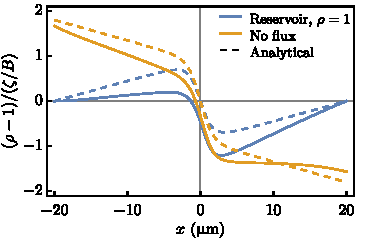
\includegraphics[width=\linewidth]{rho1d_Dirichlet_Neumann}\\
{\scriptsize solid: numerics;\; dashed: closed forms}

\vspace{1ex}
either way, only at order $\zeta/B$
\end{columns}
\backto{m-steady}
\note{Backup. No boundary at a finite distance describes a defect in an extended colony. The reservoir and the no-flux wall change the density across the disk with opposite slopes, but only at order $\zeta/B$, far below the fluctuations. A free density at the wall has no steady state.}
\end{frame}


\begin{frame}[t,label=b-cutoff]{Backup: the modulation depends on the cutoff}
\small\setlength{\abovedisplayskip}{3pt}\setlength{\belowdisplayskip}{3pt}
\begin{columns}[T,totalwidth=\textwidth]
\column{0.5\textwidth}
small $\elln$:
\[\nu_0\simeq\elln^2\Big[\tfrac14\max\big|\partial_i\partial_jQ^\ss_{ij}\big|\,\ln\frac{\elld}{\elln}+c\Big]\;\to\;0\]
\begin{itemize}\setlength{\itemsep}{0.8ex}
\item $\nu_0=2.94\%$ at $\elln=0.5~\micron$ (Pad\'e profile)
\item the peak moves away from the core as $\elln$ grows
\item the modulation exists only because the density is resolved at the width of a cell: $\elln$ is physical
\end{itemize}
\column{0.5\textwidth}
\centering
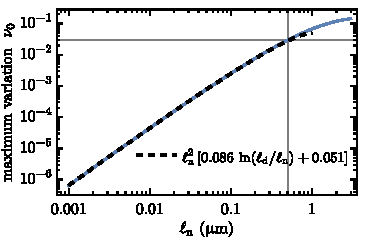
\includegraphics[width=\linewidth]{ln_curve}
\end{columns}
\backto{m-pedestal}
\note{Backup. The weight $\Omega$ reaches over a distance proportional to $\ell_\text{n}$, so the peak modulation decreases with the cutoff and vanishes at $\ell_\text{n}=0$. This makes $\ell_\text{n}$, the shortest length of the model, a physical parameter.}
\end{frame}


\begin{frame}[t,label=b-force]{Backup: fluctuations of the active force}
\small
\begin{columns}[T,totalwidth=\textwidth]
\column{0.52\textwidth}
\centering
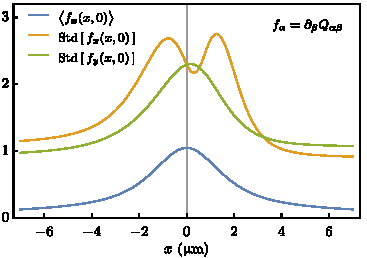
\includegraphics[width=0.88\linewidth]{fActiveMeanAndStd}\\
{\scriptsize along the axis; the active force is $-\zeta\bs f$}
\column{0.46\textwidth}
\centering
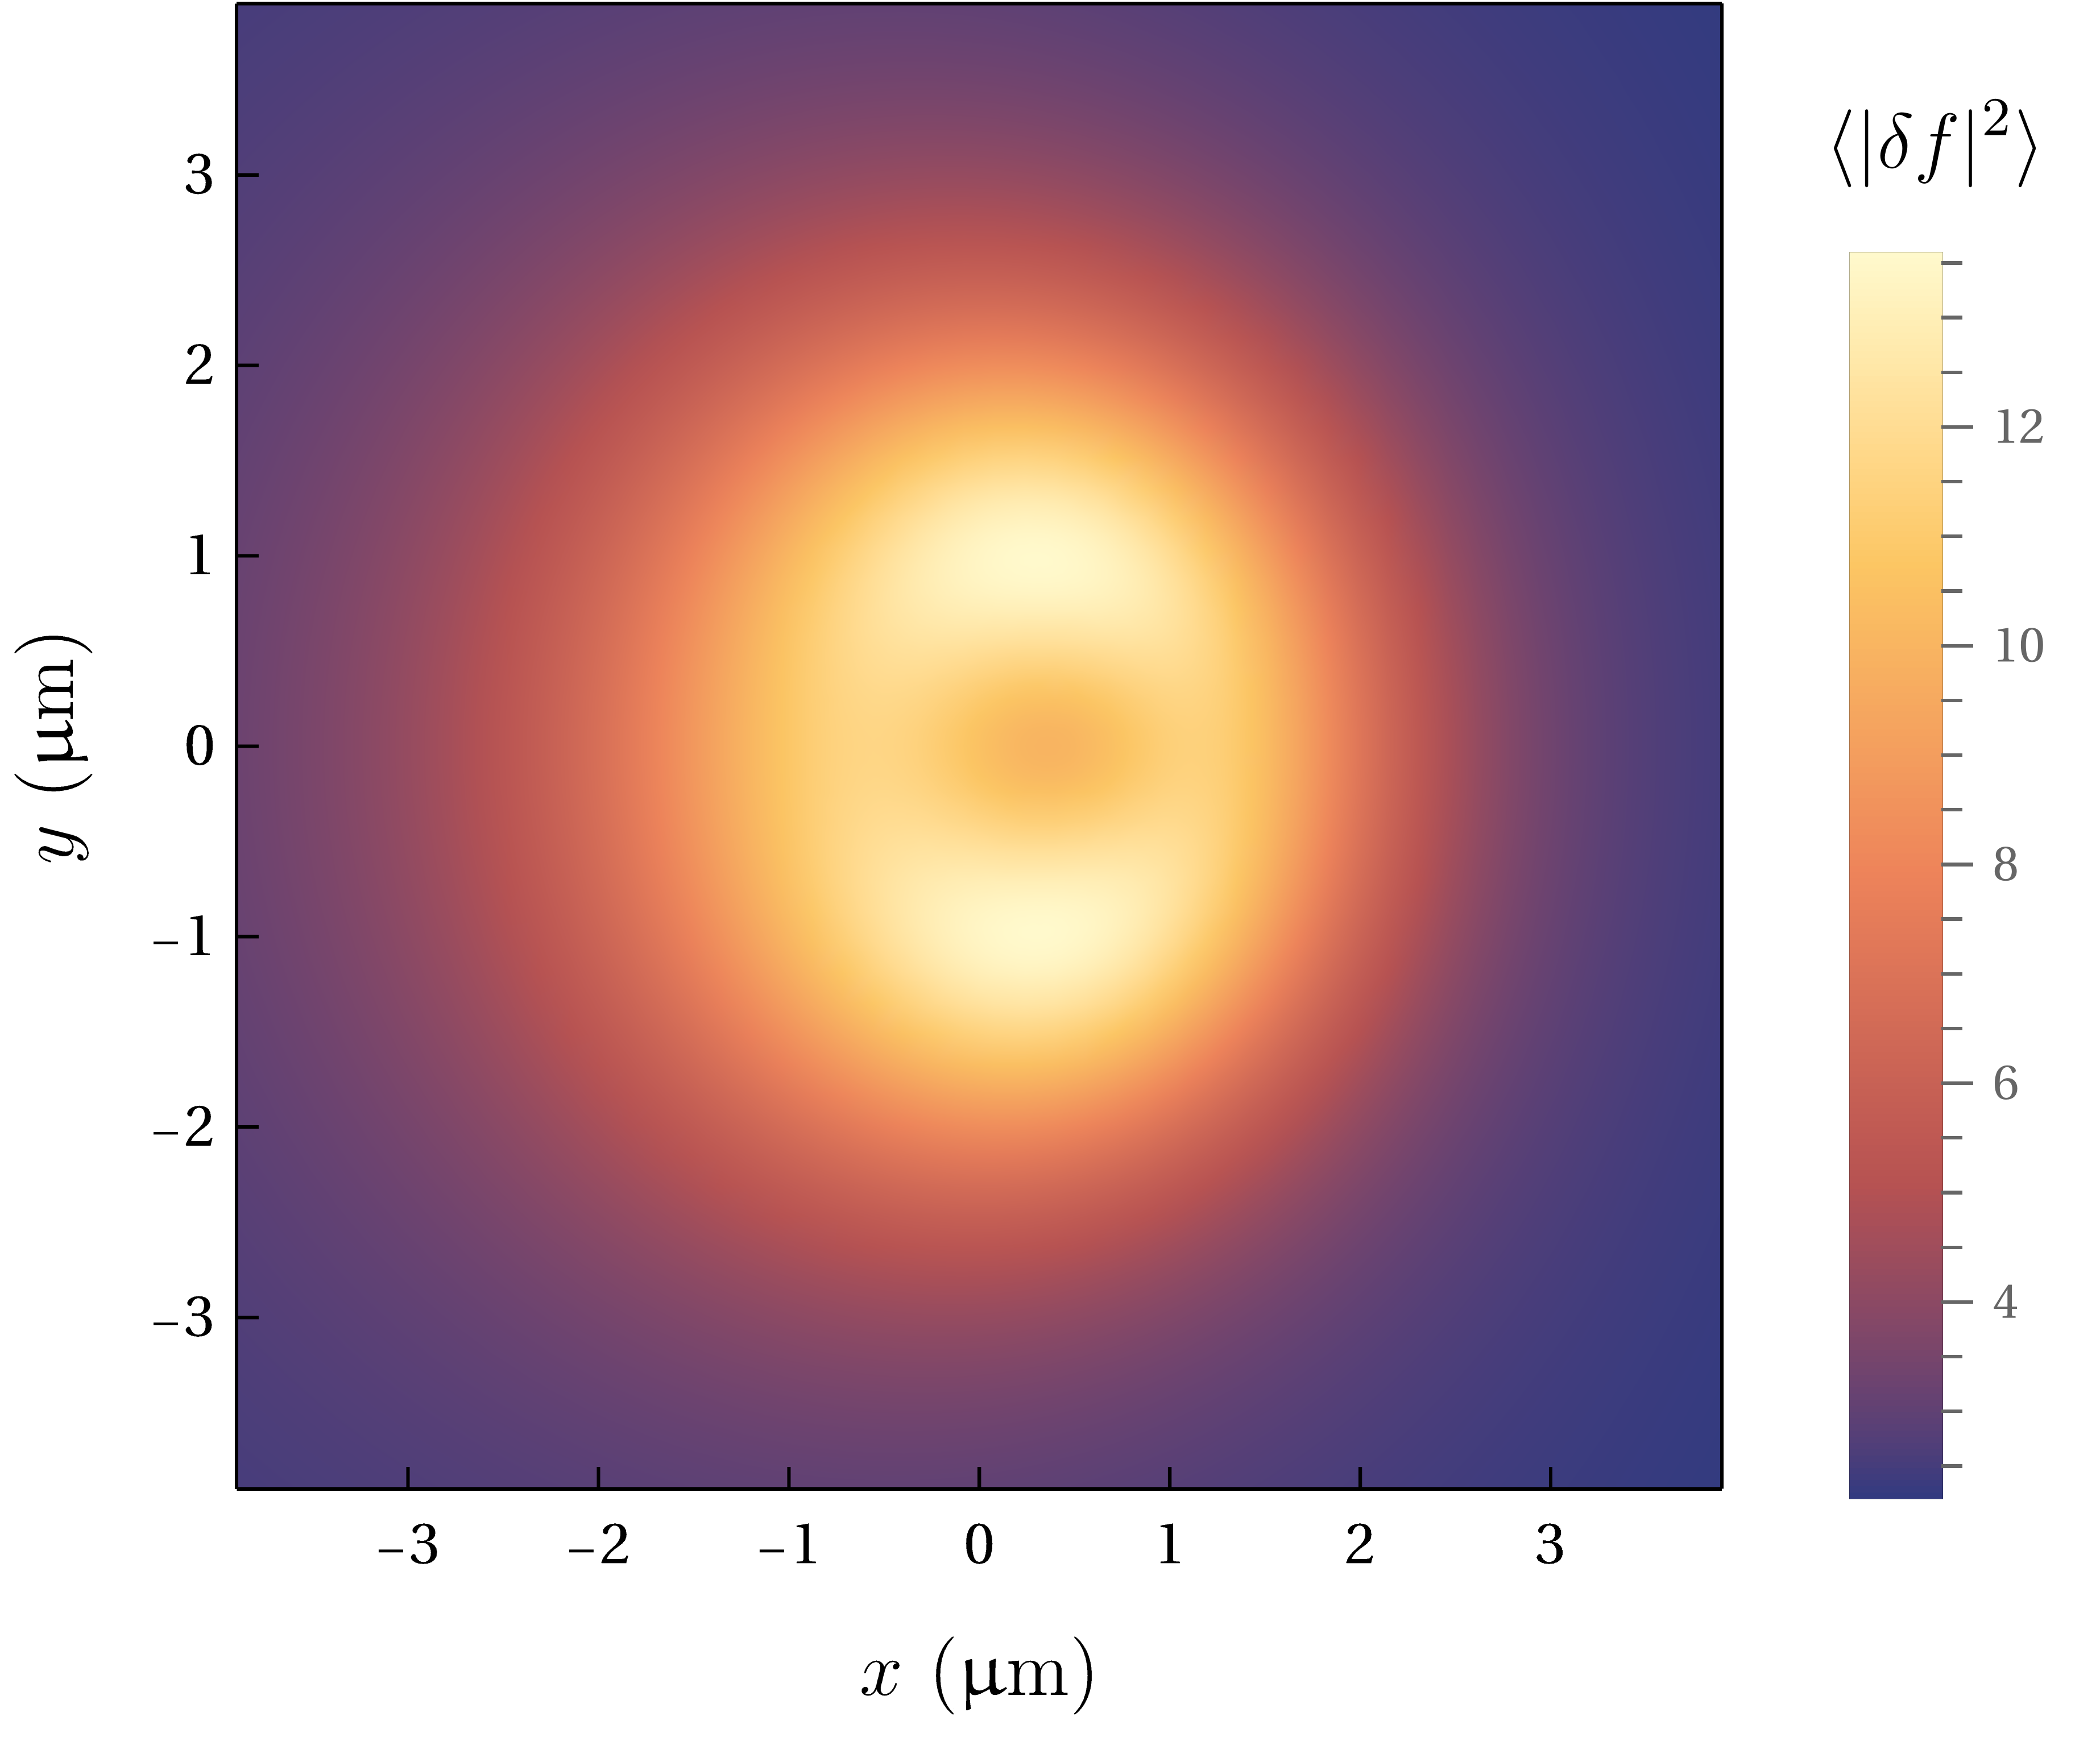
\includegraphics[width=0.62\linewidth]{f2_high}\\
{\scriptsize $\la|\delta\bs f|^2\ra$ ($\micron^{-2}$)}
\end{columns}

\vspace{0.5ex}
\footnotesize
\begin{itemize}\setlength{\itemsep}{0.2ex}
\item fluctuations exceed the mean everywhere along the axis, increasingly away from the core
\item around the core the force fluctuates mostly along the axis of the defect
\item the measured traction also contains the pressure gradient: the resemblance is qualitative
\end{itemize}
\backto{m-tests}
\note{Backup. The fluctuations of the nematic order carry fluctuations of the active force, which the analytic variance drops. They exceed the mean everywhere along the axis, a few times near the core and more away from it, where the mean decays. This resembles the measured traction, but the traction also contains the pressure gradient.}
\end{frame}


\begin{frame}[t,label=b-estimate]{Backup: first-order estimate of the drift}
\small\setlength{\abovedisplayskip}{3pt}\setlength{\belowdisplayskip}{3pt}
project the $\Q$ equation onto the translation mode $\partial_x\Psi_0$ of the static defect:
\[u_x\simeq-\frac{\la\partial_x\Psi_0,s\ra}{\la\partial_x\Psi_0,\partial_x\Psi_0\ra},\qquad
s=\frac{B}{\xi_0}\nabla\cdot(\Q\nabla\rho)+w\,\Y\]
\[u_x\simeq u_a+w\,u_b,\qquad u_a=0.28~\micron/\minute\ \text{(cross-coupling)},\qquad u_b=-0.51~\micron/\minute\ (\Y)\]
\centering{\footnotesize on a disk of radius $R=20~\micron$}\par\raggedright
\begin{itemize}\setlength{\itemsep}{0.8ex}
\item denominator $\propto S_0^2\ln(R/\elld)$: the drift slows as the boundary moves away
\item transports vs.\ relaxation: ratio $0.45$, so the estimate gives the trend, not the value
\item anisotropic friction $\xi_0(\I-\varepsilon\hat\Q)$ \refs{[Copenhagen 2021]}: only harmonics $\ee^{\pm\ii\phi}$, $\ee^{\pm3\ii\phi}$,\\ which do not project on the translation mode $\Rightarrow$ no change of the drift at first order
\end{itemize}
\backto{m-reverse}
\note{Backup. At first order in the two transports, projecting onto the translation mode of the defect gives the drift as a sum of the two contributions, linear in $w$. The estimate reverses the drift before $w$ reaches one, and overshoots the numerics. The anisotropic friction of Copenhagen et al.\ does not reverse the drift at this order.}
\end{frame}

\end{document}
